\documentclass[11pt,a4paper]{article}
\usepackage[utf8]{inputenc}
\usepackage[dvipsnames]{xcolor}
\usepackage[english]{babel}
\usepackage{listings}
\usepackage{multirow}
\usepackage{color}
\usepackage[ruled,vlined]{algorithm2e}
\renewcommand*{\thefootnote}{\fnsymbol{footnote}}
\usepackage{mathrsfs}
\usepackage{hyperref}
\usepackage{adjustbox} %adjust boxe til den rigtige størrelse
 \usepackage{biblatex} %Imports biblatex package
\addbibresource{sample.bib} %Import the bibliography file

\lstset{ %
  language=R,                     % the language of the code
  basicstyle=\footnotesize,       % the size of the fonts that are used for the code
  numbers=left,                   % where to put the line-numbers
  numberstyle=\tiny\color{gray},  % the style that is used for the line-numbers
  stepnumber=1,                   % the step between two line-numbers. If it's 1, each line
                                  % will be numbered
  numbersep=5pt,                  % how far the line-numbers are from the code
  backgroundcolor=\color{white},  % choose the background color. You must add \usepackage{color}
  showspaces=false,               % show spaces adding particular underscores
  showstringspaces=false,         % underline spaces within strings
  showtabs=false,                 % show tabs within strings adding particular underscores
  frame=single,                   % adds a frame around the codehttps://da.overleaf.com/project/5e42ac84ac4e640001f94558
  rulecolor=\color{black},        % if not set, the frame-color may be changed on line-breaks within not-black text (e.g. commens (green here))
  tabsize=2,                      % sets default tabsize to 2 spaces
  captionpos=b,                   % sets the caption-position to bottom
  breaklines=true,                % sets automatic line breaking
  breakatwhitespace=false,        % sets if automatic breaks should only happen at whitespace
  title=\lstname,                 % show the filename of files included with \lstinputlisting;
                                  % also try caption instead of title
  keywordstyle=\color{blue},      % keyword style
  commentstyle=\color{ForestGreen},   % comment style
  stringstyle=\color{mauve},      % string literal style
  escapeinside={\%*}{*)},         % if you want to add a comment within your code
  morekeywords={*,...}            % if you want to add more keywords to the set
}
\usepackage{amsmath}
\usepackage{graphicx}
\usepackage{capt-of}
\usepackage{import}
\usepackage{booktabs, array}
\usepackage{siunitx}
\usepackage{tabularx}
\usepackage{dcolumn}
\usepackage{longtable}
\usepackage{amssymb}
\usepackage{arydshln}
\usepackage{titlesec}
\graphicspath{ {pictures/} }
\addto\captionsenglish{
    \renewcommand*\contentsname{Table of Contents}
}
\usepackage{wrapfig}
\usepackage{lineno, blindtext}
\usepackage{helvet}
\usepackage{longtable}
\usepackage{fullpage}
\def\DU#1{\underline{\underline{#1}}}
\def\SU#1{\underline{#1}}
\definecolor{mygreen}{rgb}{0,0.6,0}
\usepackage{listings}
\usepackage{ulem}

\begin{document}
\begin{titlepage} % Suppresses displaying the page number on the title page and the subsequent page counts as page 1
	\newcommand{\HRule}{\rule{\linewidth}{0.5mm}} % Defines a new command for horizontal lines, change thickness here
	
	\center % Centre everything on the page
	
	%------------------------------------------------
	%	Headings
	%------------------------------------------------
	
	\textsc{\LARGE Copenhagen Business School}\\[1.5cm] % Main heading such as the name of your university/college
	
	\textsc{\Large Statistik}\\[0.5cm] % Major heading such as course name
	
	\textsc{\large Bachelorprojekt}\\[0.5cm] % Minor heading such as course title
	
	%------------------------------------------------
	%	Title
	%------------------------------------------------
	
	\HRule\\[0.4cm]
	
	{\huge\bfseries En Generalisering af Bradley-Terry Modellen og Parameter Estimering vha. LASSO}\\[0.4cm] % Title of your document
	
	\HRule\\[1.5cm]
	
	%------------------------------------------------
	%	Author(s)
	%------------------------------------------------
	
	\begin{minipage}{0.4\textwidth}
		\begin{flushleft}
			\large
			\textit{Forfattere}\\
			Lucas Johan Boesen\\ % Your name
			Christoffer Bolvig Birch\\ % Your name
			Victor Emil Skov Lundmark\\ % Your name
		\end{flushleft}
	\end{minipage}
	~
	\begin{minipage}{0.4\textwidth}
		\begin{flushright}
			\large
			\textit{Professor}\\
			\textsc{Søren Feodor Nielsen}\\
			\textsc{}\\
			\textsc{}\\% Supervisor's name
		\end{flushright}
	\end{minipage}
	
	% If you don't want a supervisor, uncomment the two lines below and comment the code above
	%{\large\textit{Author}}\\
	%John \textsc{Smith} % Your name
	
	%------------------------------------------------
	%	Date
	%------------------------------------------------
	
	\vfill\vfill\vfill % Position the date 3/4 down the remaining page
	
	{\large{December 20, 2019}} % Date, change the \today to a set date if you want to be precise
	
	%------------------------------------------------
	%	Logo
	%------------------------------------------------
	
	%\vfill\vfill
	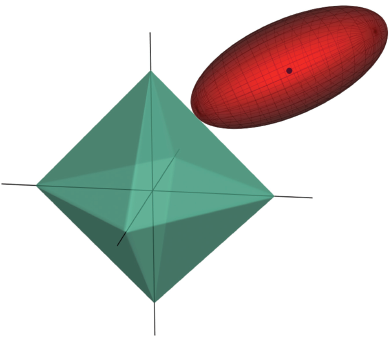
\includegraphics[width=0.7 \textwidth]{GLR2.png}\\[1cm] % Include a department/university logo - this will require the graphicx package
	 
	%----------------------------------------------------------------------------------------
	
	\vfill % Push the date up 1/4 of the remaining page
	
\end{titlepage}
\renewcommand{\contentsname}{Indholdsfortegnelse}
\clearpage
\tableofcontents
\clearpage
\newpage
\pagenumbering{arabic}
\begin{abstract}
\textcolor{blue}{English} Lynhurtig Bradley-Terry modellen anvendes til at lave parvise sammenligninger af f.eks. fodboldhold styrker. i den oprindelig model (Bradley \& Terry 1952) antages at der altid vil være en vinder, men da dette er en urealistisk betragtning blev modellen udvidet (Rao-Kupper 1967). til at inkludere en grænseværdiparameter som gør det muligt at indrage udfaldet uafgjort. Dette papir tager udgangspunkt i denne model og betragter anvendelsen af LASSO optimering til udvælgelsen af parametre til estimering af de forskellige holds styrke. 
\end{abstract}
\section{Generalisering af Bradley-Terry Modellen}
\textit{“An idea is always a generalization, and generalization is a property of thinking. To generalize means to think”} - Georg Wilhelm Friedrich Hegel
\subsection{Indledning}
Bradley og Terry (1952) introducerer en statistisk model til at rangere f.eks. forbrugervurderinger af produkter eller styrker af fodboldhold ved parvise sammenligninger. Dette gøres ved at estimere nogle nytter for produkterne eller styrker af fodboldholdene. I førstnævnte eksempel vil modellen yderligere kunne bruges til at estimere sandsynligheden for, at en forbruger foretrækker ét produkt, over et andet - i sidstnævnte eksempel til at estimere sandsynligheden for, at Brøndby vinder over FCK i deres næste opgør. I denne artikel tager vi udgangspunkt i eksemplet med sammenligninger af fodboldhold. 

\subsection{Bradley-Terry Modellen}
\textcolor{red}{W: Omskriv så det er mere klart hvd i og j er}Når vi sammenligner hold \textit{i} med hold \textit{j}, betragter vi altid situationen $i<j$, hvor vi definerer \\$i \in \{1,..,h-1\}$ og $j\in \{i+1,...,h\}$ hvor $h\in \mathbb{Z}^+$ betegner antal hold. På denne måde undgår vi at gentage parvise sammenligninger mellem hold \textit{i} og hold \textit{j}, samt at sammenligne hold med sig selv.\\
\textcolor{blue}{BT skriver} Sandsynligheden for at hold \textit{i} vinder over hold \textit{j} skrives op på formen:

\begin{align*}
    P(i\ vinder\ over\ j) = p_{i\cdot ij} = \frac{\pi_i}{\pi_i+\pi_j},
\end{align*}
hvor $p_{i\cdot ij}$ betegner sandsynligheden for at hold \textit{i} vinder over hold \textit{j}. Vi tolker $\pi_i$ og $\pi_j$ som hold \textit{i} og \textit{j}'s respektive styrker. Dermed kan $Y_i=\pi_i+\epsilon_i$ betegne hold \textit{i}'s dagsform, hvor $\epsilon_i$ er fejlled. Dette medfører hold \textit{i} vinder over hold \textit{j}, hvis $Y_i>Y_j$.\\ \textcolor{blue}{Eftersom modellens parametre kan skaleres op uden at de påvirker sandsynlighederne ses modellen at være overparameteriseret på grund af skala-invarians.} Vi kan dermed ikke identificere de enkelte styrkeparametre, men vi kan identificere forholdet mellem to styrkeparametre. For at overkomme dette problem kan der lægges et bånd på, der sikrer, at vi kan estimere styrkeparametrene; dette kan gøres i form af $\pi_1 = 0$ eller $\sum_i^n \pi_i = 1$. \\
Ved omskrivning af $p_{i\cdot ij}$ kan vi udtrykke dette styrkeforhold som:
\begin{align*}
    p_{i\cdot ij} &= \frac{\pi_i}{\pi_i+\pi_j}=\frac{1}{1+\frac{\pi_j}{\pi_i}}=\frac{1}{1+e^{-(\log(\pi_i)-\log(\pi_j))}}\\
    &=F(V_{i\cdot ij})=\int_{-\infty}^{V_{i\cdot ij}} \frac{\partial p_{i\cdot ij}}{\partial V_{i\cdot ij}} \text{ d}V=\frac{1}{1+e^{-V_{i\cdot ij}}},
\end{align*}
hvor $V_{i\cdot ij}=\log(\pi_i)-\log(\pi_j)$ beskriver log-styrken for hold \textit{i} i forhold til hold \textit{j}. Det ses altså at sandsynligheden for at \textit{i} vinder over \textit{j} afhænger af forskellen i hold \textit{i} og hold \textit{j}'s styrker. Eftersom 
\begin{align*}
&f(V_{i\cdot ij})=\frac{\partial p_{i\cdot ij}}{\partial V_{i\cdot ij}} = \frac{e^{-V_{i\cdot ij}}}{(e^{-V_{i\cdot ij}}+1)^2} \geq 0, \\ \intertext{samt at}
&\int_{-\infty}^\infty f(V_{i\cdot ij}) \text{  d} V_{i\cdot ij} = 1,
\end{align*}
er $f(V_{i\cdot ij})$ en tæthed for den logistiske fordeling, hvor $F(V_{i\cdot ij})$ er den tilhørende fordelingsfunktion, som for givne styrke parametre, kan opfattes som en sandsynlighed.\\
Sandsynligheden for at hold \textit{i} vinder over hold \textit{j} på en given kampdag, tolkes som sandsynligheden for at hold \textit{i}'s dagsform er bedre (større) end hold \textit{j}'s:
\begin{align*}
p_{i\cdot ij}&=P\big{\{}Y_i>Y_j\big{\}}
\\&=P\big{\{}(\pi_i-\pi_j)+(\epsilon_i-\epsilon_j)>0\big{\}}
\\&=P\big{\{}(\epsilon_i-\epsilon_j)>(\pi_j-\pi_i)\big{\}}
\\&=\frac{1}{1+e^{-(log(\pi_i)-log(\pi_j))}} 
\\&=\frac{\pi_i}{\pi_i+\pi_j},\;\;
\end{align*}
\\
For at forskellene mellem fejlledene $\epsilon_i-\epsilon_j$ er logistisk fordelt skal $\epsilon_i$'erne være uafhængige og gumbel fordelte.

\subsection{Rao-Kupper Modellen}
Indtil videre har det været en antagelse at en fodboldkamp altid har haft en vinder, men dette er ikke en realistisk antagelse, da fodboldkampe kan ende uafgjort. Det samme gælder forbrugervalget mellem to produkter. Realistisk set, kan en forbruger godt være ligeglad ved valget mellem to produkter, hvis produkterne giver \sout{ham/hende} \textcolor{blue}{forbrugeren} tilnærmelsesvist den samme nytte. Rao og Kupper (1967) \cite{RaoKupper} foreslår en løsning på dette dilemma; at udvide Bradley-Terry modellen med et grænseværdiparameter $\theta$. $\theta$ betegner den forskel i dagsform der mindst skal være mellem to hold, for at der er en vinder; hvis $\|Y_i-Y_j\| < \theta$ bliver kampen uafgjort. Rao-Kupper opskrives som integralet af en tæthed ligesom Bradley-Terry, og giver sandsynlighederne:
\begin{equation}
\begin{split}
    p_{i\cdot ij}&=F(V_{i\cdot ij}-\eta)=\frac{\pi_i}{\pi_i+\theta \pi_j}\\
    p_{j\cdot ij}&=F(V_{j\cdot ij}-\eta)=1-F(V_{i\cdot ij}+\eta)=\frac{\pi_j}{\theta \pi_i+\pi_j}\\
    p_{0\cdot ij}&=F(V_{i\cdot ij}+\eta)-F(V_{i\cdot ij}-\eta)= \frac{\pi_i \pi_j(\theta^2 -1)}{(\pi_i+\theta \pi_j)(\theta \pi_i + \pi_j)} \label{Sandynligheder},
\end{split}
\end{equation}
hvor $\eta=\log(\theta)>0 \rightarrow\theta>1$ og $p_{0\cdot ij}$ er sandsynligheden for det nye udfald, uafgjort. De tre udfald er direkte sammenlignelige med et rangeringssytem, da hvert af udfaldende ikke giver samme antal point; sejr = 3 point, uafgjort = 1 point og tab = 0 point. Ligeledes kan dette overføres til rangering af produktsammenligninger; bedre, ligeglad og dårligere. 

\subsection{Parameter Estimering}
\textcolor{blue}{Evt. noget intro tekst}
\textcolor{blue}{Rao-Kupper er en delmodel af den almindelige multinomialfordelingsmodel.}\\
Lad $X_{ij}$ være en tredimensionel uafhængig stokastisk variabel, som repræsenterer en kamp mellem hold \textit{i} og hold \textit{j}. $X_{ij}$'s, tilhørende udfaldsområde er dermed givet ved $(X_{i\cdot ij},\;X_{j\cdot ij},\;X_{0\cdot ij})$, som hhv. repræsenterer sejr til hold \textit{i}, sejr til hold \textit{j} og uafgjort, hvor: 
\begin{align*}
   &P\{X_{ij}=X_{i\cdot ij}\}=p_{i\cdot ij} &&P\{X_{ij}=X_{j\cdot ij}\}=p_{j\cdot ij} &&P\{X_{ij}=X_{0\cdot ij}\}=p_{0\cdot ij}
\end{align*}
\textcolor{blue}{Yderligere lader vi $r_{ij}$ være antal gentagelser af $X_{ij}$ (antal kampe mellem hold $i$ og hold $j$) for et givet tidspunkt, samt $Y_{ij}=(Y_{i\cdot ij},Y_{j\cdot ij},Y_{0\cdot ij})$ være den tilhørende kontingenstabel givet ved:}\\
\begin{align*}
    &Y_{i\cdot ij}=\sum_{k=1}^{r_{ij}}1_{\{X_{ijk}=X_{i\cdot ij}\}} &&Y_{j\cdot ij}=\sum_{k=1}^{r_{ij}}1_{\{X_{ijk}=X_{j\cdot ij}\}} &&Y_{0\cdot ij}=\sum_{k=1}^{r_{ij}}1_{\{X_{ijk}=X_{0\cdot ij}\}}
\end{align*}
\\
Til at estimere styrkeparametrene og $\theta$, vil vi gøre brug af maksimering af likelihooden, hvor likelihood-funktionen opstilles ved multinomialfordelingen med sandsynlighederne fra (\ref{Sandynligheder}). Likelihooden for de observerede udfald bliver dermed:
\begin{align*}
\mathcal{L}(\pi_1,...,\pi_h,\theta) &= \prod_{i<j}p_{i\cdot ij}^{Y_{i\cdot ij}}p_{j\cdot ij}^{Y_{j\cdot ij}}p_{0\cdot ij}^{Y_{0\cdot ij}}\\
&= \prod_{i<j}\Big{(}\frac{\pi_i}{\pi_i+\theta\pi_j}\Big{)}^{Y_{i\cdot ij}}
\;\Big{(}\frac{\pi_j}{\pi_j+\theta\pi_i}\Big{)}^{Y_{j\cdot ij}}
\Big{(}\frac{(\theta^2-1)\pi_i \pi_j}{(\pi_i+\theta\pi_j)(\pi_j+\theta\pi_i)}\Big{)}^{Y_{0\cdot ij}}\\
&=\prod_{i<j}\Big{(}\frac{\pi_i}{\pi_i+\theta\pi_j}\Big{)}^{Y_{i\cdot ij}}
\;\Big{(}\frac{\pi_j}{\pi_j+\theta\pi_i}\Big{)}^{Y_{j\cdot ij}}
\Big{(}\frac{(\theta^2-1)\pi_i \pi_j}{(\pi_i+\theta\pi_j)(\pi_j+\theta\pi_i)}\Big{)}^{r_{ij}-{Y_{i\cdot ij}}-{Y_{j\cdot ij}}}\\
\end{align*}
\textcolor{blue}{Sidstnævnte omskrivelse er tilføjet for at lette notationer, samt lette udledninger af afledte.}
Vi opskriver log-likelihooden, da vi ikke ser nogen god grund til ikke at gøre det: 
\begin{align*}
\textit{l}(\pi,\theta)
&=\sum_{i<j}\Big{[}Y_{i\cdot ij}\log\Big{(}\frac{\pi_i}{\pi_i+\theta\pi_j}\Big{)}
+ Y_{j\cdot ij}\log\Big{(}\frac{\pi_j}{\pi_j+\theta\pi_i}\Big{)}\\
&+ (r_{ij}-Y_{i\cdot ij}-Y_{j\cdot ij}) \log\Big{(}\frac{(\theta^2-1)\pi_i \pi_j}{(\pi_i+\theta\pi_j)(\pi_j+\theta\pi_i)}\Big{)}\Big{]}
\end{align*}
Som log-likelihooden ser ud i ovenstående, er der ikke noget der hindrer negative styrker. Dog er det klart at et forhold mellem en negativ styrke og en positiv styrke vil være misvisende, hvorfor vi log-transformerer styrkerne ved at sætte $\gamma_i=\log(\pi_i)$ og $\gamma_j=\log(\pi_j)$:\\
\begin{align*}
\textit{l}(\gamma,\theta)
&=\sum_{i<j}\Big{[}Y_{i\cdot ij}\Big{(}\gamma_i-\log(e^{\gamma_i}+\theta e^{\gamma_j})\Big{)}
+Y_{j\cdot ij}\Big{(}\gamma_j-\log(e^{\gamma_j}+\theta e^{\gamma_i})\Big{)}\\
& +(r_{ij}-Y_{i\cdot ij}-Y_{j\cdot ij}) \Big{(} \log(\theta^2-1)+\gamma_i+\gamma_j-\log(e^{\gamma_i}+\theta e^{\gamma_j})-\log(e^{\gamma_j}+\theta e^{\gamma_i})\Big{)}
\end{align*}
For at bestemme maksimum-likelihood estimaterne for vores parametre, har vi valgt at gøre brug af den iterative metode, Newton-Raphson. Newton-Raphson opstilles på følgende form, med den observerede information og scorefunktionen:
\begin{align*}
v_{k+1} = v_{k} + \textit{i}(v_{k})^{-1}\textit{S}(v_{k})\omega,
\end{align*}
hvor $v_{k}$ er en vektor bestående af vores styrkeparametre, $\pi_i$, samt $\theta$ og $\omega$ er skridtlængden. Eftersom parvise sammenligninger i praksis, afhænger af den data der er indsamlet, vil det være nødvendigt at have et udtryk for likelihooden i form af den data der er indsamlet. For at gøre dette, definerer vi et udtryk for samtlige $\log( \pi_i)$'er (også for referencegruppen). Dette indses ved indsættelse i den lineære sammenhæng mellem styrkerne:
\begin{align*}
    p_{i\cdot ij} = \frac{1}{1+ e^{-(log(\pi_i)-log(\pi_j))}} = \frac{1}{1+ e^{-\beta(x_i^T-x_j^T)}},
\end{align*}
hvor $x_i$ er den i'te søjle i designmatricen og $\beta$ er vores parametervektor. Designmatricens \textit{i}'te søjle indeholder altså data for hold \textit{i}, hvor den \textit{k}'te række indeholder data til den \textit{k}'te parameter i parametervektoren $\beta$. \\
I vores tilfælde vil det være data der beskriver to fodboldhold, men formen vil forblive uændret hvis det er to forbrugerprodukter der bliver sammenlignet.
%########################################################################
%\textcolor{olive}{Vi skal her overveje, om vi hellere vil skrive pseudo algoritme, med %de afledte ift, log($\pi_i$) istedet. Vi skal efterfølgende kommentere på de betingelser %der skal være opfyldt, for at vi ved at vores algoritme rent faktisk finder MLE %estimaterne.}
%\subsection{Numerisk Estimation af parametre vha. MM-algoritme}
%Estimationen af styrkeparametrene samt $\theta$
Til at implementere dette forhold i log-likelihooden, som vi skal maksimere ud fra parametrerne, indsætter vi $\gamma_i=x_i^T\beta$ og $\gamma_j=x_j^T\beta$:
\begin{align*}
\textit{l}(\beta,\theta)
&=\sum_{i<j}\Big{[}Y_{i\cdot ij}\Big{(}x_i^T\beta-\log(e^{x_i^T\beta}+\theta e^{x_j^T\beta})\Big{)}
+Y_{j\cdot ij}\Big{(}x_j^T\beta-\log(e^{x_j^T\beta}+\theta e^{x_i^T\beta})\Big{)}\\
& +(r_{ij}-Y_{i\cdot ij}-Y_{j\cdot ij}) \Big{(} \log(\theta^2-1)+x_i^T\beta+x_j^T\beta-\log(e^{x_i^T\beta}+\theta e^{x_j^T\beta})-\log(e^{x_j^T\beta}+\theta e^{x_i^T\beta})\Big{)}\Big{]}
\end{align*}
Førsteordensbetingelserne til scorefunktionen for $\beta$ og $\theta$ bliver:
\begin{align*}
\frac{\partial \ell(\beta;\theta)}{\partial \beta}&= 
\sum_{i<j}\Big{[}\Big{(}
(r_{ij}-Y_{i\cdot ij})\Big{(}-\frac{\theta e^{x_i^T\beta}}{e^{x_j^T\beta}+\theta e^{x_i^T\beta}}\Big{)}+(r_{ij}-Y_{j\cdot ij})\Big{(}\frac{\theta e^{x_j^T\beta}}{e^{x_i^T\beta}+\theta e^{x_j^T\beta}}\Big{)}\Big{)}(x_i-x_j)\Big{]},\\
\frac{\partial \ell(\beta;\theta)}{\partial \theta}&=
\sum_{i<j}
\Big{[}
 (r_{ij}-Y_{i\cdot ij}-Y_{j\cdot ij})\Big{(}\frac{2\theta}{\theta^2-1}\Big{)}\\
 &+(r_{ij}-Y_{i\cdot ij})\Big{(}-\frac{e^{x_i^T\beta}}{\theta e^{x_i^T\beta}+e^{x_j^T\beta}}\Big{)}
 +(r_{ij}-Y_{j\cdot ij})\Big{(}-\frac{e^{x_j^T\beta}}{e^{x_i^T\beta}+\theta e^{x_j^T\beta}}\Big{)}
\Big{]},\\
\end{align*}
hvor førsteordensbetingelsen ift. $\beta$ bliver en vektor med længden lig antal rækker i designmatricen. Dermed kan scorefunktionen opstilles som:
\begin{equation}
S(\beta,\theta) = \begin{bmatrix}
\frac{\partial \ell(\beta;\theta)}{\partial \beta}\\
\frac{\partial \ell(\beta;\theta)}{\partial \theta}
\end{bmatrix}
\label{score}
\end{equation}

Udledningerne til andensordsbetingelserne bliver ligeledes: 
\begin{align*}
\frac{\partial^2 \ell(\beta;\theta)}{\partial \beta^2}
&= \sum_{i<j}\Big{[}\Big{(} -\frac{(r_{ij}-Y_{i\cdot ij})}{(\theta e^{x_i^T\beta}+e^{x_j^T\beta})^2}-\frac{(r_{ij}-Y_{j\cdot ij})}{(e^{x_i^T\beta}+\theta e^{x_j^T\beta})^2}\Big{)}e^{x_i^T\beta+x_j^T\beta}\theta(x_{i}-x_{j})^2 \Big{]},\\
\frac{\partial^2 \ell(\beta;\theta)}{\partial \theta^2}
&= \sum_{i<j} 
\Big{[}
(r_{ij}-Y_{i\cdot ij}-Y_{j\cdot ij})\Big{(}-\frac{2(\theta^2+1)}{(\theta^2-1)^2}\Big{)}\\
&+(r_{ij}-Y_{i\cdot ij})\Big{(}\frac{e^{2x_i^T\beta}}{(\theta e^{x_i^T\beta}+e^{x_j^T\beta})^2}\Big{)}
+(r_{ij}-Y_{j\cdot ij})\Big{(}\frac{e^{2x_j^T\beta}}{(e^{x_i^T\beta}+\theta e^{x_j^T\beta})^2}\Big{)}\Big{]},
\\
\frac{\partial^2 \ell(\beta;\theta)}{\partial \beta\partial \theta}
&= \sum_{i<j}\Big{[}\Big{(}
-\frac{(r_{ij}-Y_{i \cdot ij})}{(\theta e^{x_i^T\beta}+e^{x_j^T\beta})^2}
+\frac{(r_{ij}-Y_{j \cdot ij})}{(e^{x_i^T\beta}+\theta e^{x_j^T\beta})^2}\Big{)}e^{x_i\beta+x_j\beta}(x_{i}-x_{j})\Big{]},
\end{align*}
hvorved vi nu får at andenordensbetingelsen ift. $\beta$ bliver en kvadratisk matrice, hvorfor den observerede informationen opskrives som en symmetrisk blok-matrix på formen:
\begin{equation}
i(\beta,\theta) = -\begin{bmatrix}
\frac{\partial^2 \ell(\beta;\theta)}{\partial \beta^2} &\frac{\partial^2 \ell(\beta;\theta)}{\partial \beta \partial \theta} \\
\Big{(}\frac{\partial^2 \ell(\beta;\theta)}{\partial \beta \partial \theta}\Big{)}^T & \frac{\partial^2 \ell(\beta;\theta)}{\partial \theta^2}
\end{bmatrix}
\label{inf}
\end{equation}
Likelihooden konvergerer mod et maksimum givet scorefunktionen (\ref{score}) og den observerede information (\ref{inf}), hvis den observerede information (\ref{inf}) er positiv semi-definit. Da $i(\beta,\theta)$ er symmetrisk kan vi benytte Albert (1969;1972)'s Theorem \\\textbf{ THEOREM 9.1.6:} \textit{Lad A være symmetrisk, så:}
\begin{flalign*}
&M = \begin{bmatrix}
A & B\\
C & D
\end{bmatrix}\geq 0 \iff &\\
&(i)\; D\geq0\\
&(ii)\; C=D^{-1}DC\\
&(iii)\; A\geq BD^{-1}C\\
\end{flalign*}  
ad (\textit{i}): 
Vi ønsker at vise; $-\frac{\partial^2 \ell(\beta;\theta)}{\partial \theta^2} \succ 0 \text{ og } \iff (r_{ij}- Y_{i\cdot ij}-Y_{j\cdot ij}) \frac{2(\theta^2+1)}{(\theta^2-1)^2}>(r_{ij}-Y_{i\cdot ij})p_{i\cdot ij}^2 + (r_{ij}-Y_{j\cdot ij})p_{j\cdot ij}^2$. Det antages, at vi har mindst én uafgjort kamp i det datasæt vi undersøger, $(r_{ij}- Y_{i\cdot ij}-Y_{j\cdot ij}) > 0$.
\\Observation I: Når $Y_{0\cdot ij}$ bliver meget lille konvergerer $\theta$ mod 1, hvilket medfører venstre siden i uligheden bliver numerisk stor. $p_{i\cdot ij}^2$ og $p_{j\cdot ij}^2$ vil også blive større, men de to kvadrerede sandsynligheder vil stadig have en sum mindre end 1.\\
Observation II: Når $Y_{0\cdot ij}$ er meget stor vil både venstre og højre side konvergere mod 0. Dette ses for venstresiden da $\theta$ går mod  $\infty$, og for højresiden da sandsynlighederne for sejr til hold $i$ og $j$ går mod 0. Hvilken af dem der vægter højest kan ikke siges uden konkrete observationer for $Y$'erne. Dog vil tilfældet hvor $Y_{0 \cdot ij}$ er større end $Y_{i \cdot ij} \text{ og } Y_{j \cdot ij}$ for mange hold, være yderst sjældent da udfaldet uafgjort ikke fremkommer så hyppigt, som de andre to tilsammen.\\
ad (\textit{ii}): Det er klart at, da $D$ er endimensionel er D altid invertibel, og dermed $D D^{-1}=1 \rightarrow C=C$.\\
ad (\textit{iii}):
Det er klart at $A$ i vores tilfælde altid vil være positiv, da $-\frac{\partial^2 \ell(\beta;\theta)}{\partial \beta^2}$ kun består af positive led.
Derudover har vi at $BD^{-1}C$ også er positiv, da $D^{-1}>0$ eftersom $D$ i vores tilfælde er endimensionelt, samt at eftersom $B$ og $C$ altid vil have samme fortegn, vil deres produkt være positivt. Hvorvidt denne ulighed er opfyldt, vil 
i høj grad komme an på fordelingen af $Y$'erne. \\\\
Det kan altså ikke konkluderes at vores observerede information er positiv semi-definit for samtlige $\theta$'er. Hvorimod $\beta$'erne for et låst $\theta$, vil konvergere, da $A$ altid er positiv. \\
For at være sikker på, at vores log-likelihood konvergerer mod et maksimum, kan der gøres en af følgende tiltag:\\
1) Finde Profillikelihooden for $\beta$'erne, hvor $\theta$ holdes fast.\\
2) For hvert skridt i Newton-Raphton tjekkes der for, om det givne $\theta$ opfylder ($i$) og ($iii$) fra theorem 9.1.6.\\
I praksis vil tiltag 2) være mere medgørelig at implementere, eftersom 1) vil kræve markant flere iterationer, da der først skal itereres over $\beta$'erne og derefter over $\theta$. Eftersom vi ikke ved præcist hvordan $\theta$ vil opføre sig, vil det være en god idé at implementere en skridthalvering. Hvis $\theta$ bevæger sig ud af mængden der ikke opfylder betingelserne, kan man iterere tilbage, hvor hvert skridt halveres yderligere, indtil vi er inde i mængden igen. Metoden til at finde profillikelihooden i praksis ville være at udføre Newton-Raphson hvor $\theta$ er i et interval, eksempelvis fra 1.01 til 2. Hvis der ikke findes et maksimum, kan man udvide dette interval.

\subsection{Hypotesetest af modellen}
Eftersom modellen skal anvendes i praksis, vil det være nødvendigt at teste den for at bekræfte, at den teoretiske model kan anvendes med en vis sikkerhed på det givne data. Det er antaget at det valgte datasæt er komplet, repræsentativt og stort. \\
På trods af at dataet er valgt ud fra forventningen om, at de beskrivende variable afspejler forholdet mellem holdenes styrker, kan dette ikke antages at være gældende. For at bekræfte at dataet er beskrivende, vil vi gøre brug af en log-likelihood ratio test på parametrene, på formen:\\
$H_0: \hat{\beta} = 0$\\
Hvis der ikke er evidens for at $\hat{\beta}$'erne er forskellige fra 0, vil det betyde, at holdenes styrker ikke har nogen indflydelse på udfaldene (da alle styrkerne vil blive ens). Vi sætter dermed vores test-statistik op, hvor log-likelihooden maksimeres ift. $\theta$ med $\hat{\beta}$ holdt fast lig 0:\\
\begin{align*}
\textcolor{blue}{Q} LR = -2\Big{(}\text{max}_\theta \;\ell (\beta_{H_0},\theta)-\ell (\beta_{MLE},\theta_{MLE})\Big{)}
\end{align*}
Her antages det, at for store stikprøver, er LR omtrent $\chi^2$-fordelt med $(k-1)$ frihedsgrader. \\
Vi undlader at teste for om $\theta=1$, da den udvidede model dermed bliver nyttesløs, eftersom udfaldet uafgjort vil være udeladt fra modellen. \\\\
\textbf{Standardfejl for de forklarende variable ($\beta$'er) og grænseværdiparameter $\theta$}.\\
Først opstilles dispersionsmatricen $\hat{\Sigma}$(kovariansmatricen): \textcolor{blue}{**Mener at fordi det er numerisk kan vi godt bruge observationen, ellers skal vi lige have beregnet fisher informationen og brugt den i stedet*** }
\begin{align*}
&\hat{\Sigma}=i(\beta,\theta)^{-1}=
\Big{(}-\begin{bmatrix}
\frac{\partial^2 \ell(\beta;\theta)}{\partial \beta^2} &\frac{\partial^2 \ell(\beta;\theta)}{\partial \beta \partial \theta} \\
\Big{(}\frac{\partial^2 \ell(\beta;\theta)}{\partial \beta \partial \theta}\Big{)}^T & \frac{\partial \ell(\beta;\theta)}{\partial \theta^2}
\end{bmatrix}\Big{)}^{-1}\\
\end{align*}
\begin{align}
\intertext{Standardfejlene $\hat{\sigma}_\beta$ og $\hat{\sigma}_\theta$ findes ved kvadratroden af diagonalen af $\hat{\Sigma}$}
\hat{\sigma}_{\beta,\theta}=\sqrt{\text{diag}(\hat{\Sigma})}=
\begin{bmatrix}
\hat{\sigma}_{\beta_1}& &\\
& \ddots & \\
& & \hat{\sigma}_{\beta_k} \\
& & & \hat{\sigma}_{\theta}
\end{bmatrix}
\end{align}
Modellen kan i sin helhed testes ved en $\chi^2$ Goodness of Fit test, hvor vi kan teste de kumulerede sandsynligheder op imod de observerede sandsynligheder fra kontingenstabellen. Vi kan opstille en kontingenstabel for de forventede udfald ud fra $\hat{Y}_{ij}(t) = (p_{i\cdot ij},p_{j\cdot ij},p_{0\cdot ij})$, som er udregnet ved brug af de estimerede $\hat{\beta}$ og $\hat{\theta}$:
%For at tjekke modellen igennem er det praktisk udregne residualerne:
\begin{align*}
&\textbf{Rå (respons) residualer  }\\
&\epsilon_{i\cdot ij}=Y_{i\cdot ij}-r_{ij}p_{i\cdot ij}
&&\epsilon_{j\cdot ij}=Y_{i\cdot ij}-r_{ij} p_{j\cdot ij}
&&\epsilon_{0\cdot ij}=Y_{0\cdot ij}-r_{ij} p_{0\cdot ij}\\
&\epsilon_{i\cdot ij}=Y_{i\cdot ij}-r_{ij} \frac{\pi_i}{\pi_i+\theta \pi_j}
&&\epsilon_{j\cdot ij}=Y_{i\cdot ij}-r_{ij} \frac{\pi_j}{\theta \pi_i+ \pi_j}
&&\epsilon_{0\cdot ij}=Y_{0\cdot ij}-r_{ij} \frac{(\theta^2-1)\pi_i\pi_j}{(\pi_i+\theta \pi_j)(\theta
\pi_i + \pi_j)}\\
\end{align*}
\begin{align*}
&\hat{Y}_{i\cdot ij} = r_{ij}\frac{e^{x_i^T\beta}}{e^{x_i^T\beta}+\theta e^{x_j^T\beta}},
&&\hat{Y}_{j\cdot ij} = r_{ij}\frac{e^{x_j^T\beta}}{e^{x_j^T\beta}+\theta e^{x_i^T\beta}},
&&\hat{Y}_{0\cdot ij} = r_{ij}\frac{(\theta^2-1)e^{x_i^T\beta}e^{x_j^T\beta}}{(e^{x_i^T\beta}+\theta e^{x_j^T\beta})(e^{x_i^T\beta}\theta +e^{x_j^T\beta})}.
\end{align*}
Vores $\chi^2$ teststørrelse bliver:
\begin{align*}
\chi^2 = \sum_{i<j} \frac{(Y_{i\cdot ij}-\hat{Y}_{i\cdot ij})^2}{\hat{Y}_{i\cdot ij}} + \frac{(Y_{j\cdot ij}-\hat{Y}_{j\cdot ij})^2}{\hat{Y}_{j\cdot ij}} + \frac{(Y_{0\cdot ij}-\hat{Y}_{0\cdot ij})^2}{\hat{Y}_{0\cdot ij}}
\end{align*}
Her vil det også gælde for tilstrækkeligt store stikprøver at teststørrelsen er $\chi^2$ fordelt, og her med $(h^2-2h)$ frihedsgrader. \\
Ovenstående tests skal evalueres med en vis forsigtighed, eftersom antagelsen om at den underliggende fordeling er logistisk, ikke altid vil være opfyldt. Derfor er det vigtigt at kigge på dem som en helhed, og ydermere ved brug af et PP-plot, hvor vi kigger på den teoretiske fordeling op imod vores estimerede udfald. 

\section{Modelovervejelser}
\subsection{Implementering af modellen}
Når det kommer til implementering af modellen, er det først og fremmest vigtigt at afklare hvad formålet med modelleringen er. Vi har valgt at stille modellen op på to forskellige måder. Den første er en statisk model, hvor styrkerne er faste over tid, hvis formål er at rangere en gruppe, af eksempelvis fodboldhold, efter respektive styrker for en given periode. Her er styrkerne udregnet ved gennemsnit af præstationer for perioden. Det var denne model (Rao og Kupper 1967) foreslog. Den anden er en dynamisk version af modellen, hvor styrkerne ændrer sig over tid, dermed kommer sandsynlighederne til at ændre sig over tid. Denne models formål er at estimere sandsynlighederne for udfaldet af en kamp mellem to hold på et givet tidspunkt. I vores eksempel med fodbold vil et tidspunkt være en spillerunde. 
\subsubsection{Statisk Model}
I den statiske model foregår rangeringen for en given periode, hvor designmatricen bliver baseret på observationer for samtlige kampe der er spillet i perioden, og er dermed faste over tid. Det medfører at styrkerne og således sandsynlighederne for at hold $i$ vinder over hold $j$ bliver faste over tid. I den statiske version bliver sandsynligheden for at hold $i$ vinder over hold $j$ for en hvilken som helst spillerunde:
\begin{align}
    \hat{p}_{i\cdot ij}=\textcolor{red}{{P\big{\{}Y_i>Y_j\big{\}}}}
    &=\frac{\hat{\pi}_i\big{(}x_i,\hat{\beta}\big{)}}{\hat{\pi}_i\big{(}x_i,\hat{\beta}\big{)}+\hat{\theta}\hat{\pi}_j\big{(}x_j,\hat{\beta}\big{)}}\\
    &=\frac{1}{1+e^{-\big{(}x_i^T\hat{\beta}-x_j^T\hat{\beta}-\hat{\eta}\big{)}}}
\end{align}
Parametrene $\hat{\beta}$ og $\hat{\theta}$ er også faste over tid, og estimeres med Newton-Rhapson algoritmen ud fra optimeringsproblemet:
\begin{align*}
\min_{\beta,\,\theta} \Big{\{}-\ell\Big{(}\beta,\theta|x,Y_{ij},R_{ij}\Big{)}\Big{\}}=
\min_{\beta,\,\theta} \Big{\{}&- \sum_{i<j}\Big{[}Y_{i\cdot ij}\log\Big{(}\frac{\pi_i}{\pi_i+\theta\pi_j}\Big{)}
+ Y_{j\cdot ij}\log\Big{(}\frac{\pi_j}{\pi_j+\theta\pi_i}\Big{)}\\
&+ \big{(}R_{ij}-Y_{i\cdot ij}-Y_{j\cdot ij}\big{)} \log\Big{(}\frac{(\theta^2-1)\pi_i \pi_j}{(\pi_i+\theta\pi_j)(\pi_j+\theta\pi_i)}\Big{)}\Big{]}\Big{\}},\\
\end{align*}
\textcolor{blue}{hvor $R_{ij}=\sum_1^n r_{ij}(t)$ er antal kampe mellem hold $i$ og hold $j$ for den givne periode og $Y_{i\cdot ij}=\sum_1^n y_{i \cdot ij}(t)$ er antal gange hold $i$ har vundet over hold $j$ i perioden, som nævnt. En periode forstås som summen af en endelig mængde tidspunkter. } hvor $\pi_i=\pi_i\big{(}x_i^T,\beta\big{)}$
\begin{algorithm}[H]
\SetAlgoLined
\KwResult{$\min_{\beta,\,\theta} \Big{\{}-\ell\Big{(}\beta,\theta|x,Y_{ij},R_{ij}\Big{)}\Big{\}}$}
 Initialisér $v_0 = \begin{bmatrix}
           \beta \\
           \theta
         \end{bmatrix} =\begin{bmatrix}
           \beta_0 \\
           \theta_0
         \end{bmatrix}\;$\\
 \For{($k = 1,2,... $ indtil konvergens)}{
  {$L(\beta_k,\theta_k) = \sum_{i<j}\ell\Big{(}\beta,\theta\Big{|}x,Y_{ij},R_{ij}\Big{)}$}\;
  $g_k = \nabla L\Big{(}\beta_k,\theta_k\Big{)}$, $j_k = -\nabla^2 L\Big{(}\beta_k,\theta_k\Big{)}$\;
  \eIf{($j_k$ er positiv semi definit)}{
   $\omega = \frac{1}{2}$\;
   }{
   $\omega = -\frac{1}{4}$\;
   }
   $v_{k+1} = v_k - j_k^{-1}g_k\omega$\;
   $v_{k+1} = \begin{bmatrix}
           \beta_{k+1} \\
           \theta_{k+1}
         \end{bmatrix}$
}
\caption{Newton-Raphson for Statisk Model}
\end{algorithm}
\subsubsection{Dynamisk Model}
Ændringen til den dynamiske model er, at designmatricen og kontingenstabellerne bliver kampspecifikke og dermed ændrer sig for hver runde. En kamp i runden $t$, vil blive beskrevet af kamppræstationer fra runder før $t$, så $t>1$ altid. Under tesen om, at et holds styrke i en given runde i højere grad afhænger af de runder, der er spillet kort forinden - fremfor samtlige runder spillet før den givne runde - tilføjer vi en tuning størrelse $\alpha$. $\alpha$ bestemmer dermed hvor mange runder før $t$ designmatricen indeholder observationer fra. Den dynamiske model åbner også op for implementering af kampspecifikke kovariater som hjemmebanefordel; disse opdateres i forhold til runden $t$. Den nye designmatrice bliver:
\begin{align*}
\textbf{X}(t,\alpha)=\begin{bmatrix}
\textbf{X}_{\text{Kategorisk}}(t)\\
\textbf{X}_{\text{Numerisk}}(t,\alpha)
\end{bmatrix}\text{,   }\textbf{X}_{\text{Numeriske}}(t,\alpha)=\sum_{k=t-\alpha}^{t-1}\textbf{x}_{\text{Numeriske}}(k),
\end{align*}
\textcolor{blue}{hvor $\textbf{X}_{\text{Kategorisk}}(t)$ beskriver de kategoriske kovariater i runden $t$ der kun afhænger af runde t, $\textbf{X}_{\text{Numerisk}}(t,\alpha)$ beskriver de numeriske kovariater i runde $t$, der opdateres for $\alpha$ tidligere runder, og $\textbf{x}_{\text{Numerisk}}(k)$ beskriver de numeriske kovariater for runde $k\in \{t-1-\alpha;t-1\}$. $\alpha\geq1$ og hvis $\alpha\geq t$ sættes $\alpha=t-1$}.
\textcolor{blue}{Dermed bliver den estimerede sandsynlighed for at hold $i$ vinder over hold $j$ i den dynamiske model:}
\begin{align*}
\hat{p}_{i\cdot ij}(t)=\textcolor{red}{P\big{\{}Y_{i}(t)>Y_{j}(t)\big{\}}}&=\frac{\hat{\pi}_i\big{(}x_i(t,\alpha),\hat{\beta}\big{)}}{\hat{\pi}_i\big{(}x_i(t,\alpha),\hat{\beta}\big{)}+\hat{\theta}\hat{\pi}_j\big{(}x_j(t,\alpha),\hat{\beta}\big{)}}\\
&=\frac{1}{1+e^{-\big{(}x_i^T(t,\alpha)\hat{\beta}-x_j^T(t,\alpha)\hat{\beta}-\hat{\eta}\big{)}}},
\end{align*}
parametrene $\hat{\beta}$ og $\hat{\theta}$ er stadig faste over tid, og bliver estimeret med Newton-Rhapson algoritmen, ud fra det nye optimeringsproblem:
\begin{align*}
\min_{\beta,\,\theta} \Big{\{}-\ell\Big{(}\beta,\theta\Big{|}x(t,\alpha),y_{ij}(t),r_{ij}(t)\Big{)}\Big{\}}=&\min_{\beta,\,\theta} \Big{\{}- \sum_{t}\sum_{i<j}\Big{[}y_{i\cdot ij}(t)\log\Big{(}\frac{\pi_i}{\pi_i+\theta\pi_j}\Big{)}
+ y_{j\cdot ij}(t)\log\Big{(}\frac{\pi_j}{\pi_j+\theta\pi_i}\Big{)}\\
&+ \big{(}r_{ij}(t)-y_{i\cdot ij}(t)-y_{j\cdot ij}(t)\big{)} \log\Big{(}\frac{(\theta^2-1)\pi_i \pi_j}{(\pi_i+\theta\pi_j)(\pi_j+\theta\pi_i)}\Big{)}\Big{]}\Big{\}},
\end{align*}
hvor $\pi_i=\pi_i\big{(}x_i^T(t,\alpha),\beta\big{)}$. $\alpha$ vælges ved at sammenligne ($\alpha=1,...,\alpha=t-1$); den størrelse der giver den største likelihood vælges. Bemærk, at $r_{ij}(t)$, $y_{i\cdot ij}(t)$ samt $y_{j\cdot ij}(t)$ er kampspecifikke {0,1}-variable og derfor ændrer sig over tid:
\begin{align*}
r_{ij}(t)&=\begin{cases}
1\text{, hvis hold $i$ spiller mod hold $j$ i runde $t$}\\
0\text{, ellers}
\end{cases}\\
y_{i\cdot ij}(t)&=\begin{cases}
1\text{, hvis hold $i$ vinder over hold $j$ i runde $t$}\\
0\text{, ellers}
\end{cases}
\end{align*}
I en spillerrunde i fodbold spiller hvert hold kun én kamp per runde; hvis hold $i$ ikke spiller mod hold $j$ i runde $t$ er $y_{i\cdot ij}=y_{j\cdot ij}=0$.\\
Til sammenligningen af de to modeller, skal det bemærkes at parameter estimaterne ikke er ens. I den dynamiske model maksimeres likelihooden, således at sandsynligheden for udfaldet af hver eneste specifik kamp maksimeres. I den statiske maksimeres likelihooden ud fra et gennemsnit af alle kampene. Således at sandsynligheden maksimeres for at hold $i$ har det sande antal sejrer, uafgjorte og tabte kampe mod hold $j$ for perioden. Der er altså ikke taget højde for rækkefølgen af kampenes udfald. Derudover vil modellerne helller ikke være baseret på præcis samme data, da den dynamiske model kræver at vi starter mindst én runde inde i perioden. Den dynamiske model \textcolor{red}{kan} også anvendes til rangering af holdene, men det må forventes, at den endelig rangering af holdene er bedre i den statiske model. \textcolor{magenta}{birchfixpls}
\begin{algorithm}[H]
\SetAlgoLined
\KwResult{$\min_{\beta,\,\theta} \Big{\{}-\ell\Big{(}\beta,\theta|x,y_{ij}(t),r_{ij}(t)\Big{)}\Big{\}}$}
 Initialisér $v_0 = \begin{bmatrix}
           \beta \\
           \theta
         \end{bmatrix} =\begin{bmatrix}
           \beta_0 \\
           \theta_0
         \end{bmatrix}\;$\\
 \For{($k = 1,2,... $ indtil konvergens)}{
  \For{$(t = 3,t\leq SlutRunde,t++)$}{
        \eIf{($\alpha\geq t$)}{$\alpha_1 = t-1\;$}{$\alpha_1 = \alpha\;$}
        $L(\beta_k,\theta_k) = \sum_{c = t-\alpha_1}^{t-1}\sum_{i<j}\ell\Big{(}\beta,\theta\Big{|}x(t,\alpha),Y_{ij}(t),R_{ij}(t)\Big{)}$\;
        $g_k = g_k + \nabla \L\Big{(}\beta_k,\theta_k\Big{)}$\;
        $j_k = j_k + (-\nabla^2 L\Big{(}\beta_k,\theta_k\Big{)})$\;
    }
   \eIf{($j_k$ er positiv semi definit)}{
   $\omega = \frac{1}{2}$\;
   }{
   $\omega = -\frac{1}{4}$\;
   }
   $v_{k+1} = v_k - j_k^{-1}g_k\omega$\;
   $\begin{bmatrix}
           \beta_{k+1} \\
           \theta_{k+1}
         \end{bmatrix} = v_{k+1}\;$
 }
\caption{Newton-Raphson for Dynamisk Model}
\end{algorithm}
\subsection{Sammenligninger af modellerne}
I denne del, vil vi teste modellen på historisk data fra den danske 3F Superliga. Superligaen er siden 2016 bestående af 14 hold, hvoraf der i hver sæson rykker ét hold op fra 1. Divison og ét hold ned til 1. Divison. Efter sæsonafslutningen i 2016 blev Superligaens opbygning ændret, og de deler derfor ligaen op i to grupper i slutspillet, hvilket medfører at alle hold ikke spiller mod hinanden lige mange gange. Det i sig selv er ikke et problem for modellen, men eftersom hvert hold kun spiller 2-3 kampe mod hinanden, giver det mest mening at tage en sæson før 2016, for at få det bedste sammenligningsgrundlag. Derfor har vi valgt at tage udgangspunkt i sæsonen 2015-2016, hvor der er 12 hold i ligaen og alle spiller det samme antal kampe mod hinanden; 198 kampe i alt. Der er i alt 33 spillerunder, hvor hvert hold spiller én kamp pr. runde.\\
Vi tester de to versioner af den udvidede Bradley-Terry model; den statiske og den dynamiske. Den statiske model tager som tidligere beskrevet udgangspunkt i det fulde datasæt, hvor designmatricen samt kontingenstabellen bliver faste. I den dynamiske model opdaterer vi designmatricen for hver runde, hvor kontingenstabellen kun indeholder udfaldene for den givne runde. Dette vil medføre at styrkerne til holdene skal evalueres for hver iteration, hvilket gør at likelihooden, scorefunktionen og den observerede information bliver evalueret antal runder flere gange for hver iteration, end de gør i den statiske model.\\
Designmatricen bliver opstillet som i Table \ref{tab:Designmatrice}, hvor vi i den statiske model undlader kovariaterne "HjemmeBane" og "streak". Designmatricen er opstillet på ligevis for den dynamiske, hvor den blot ændrer sig for hver runde, som set i \textit{Algorithm 2}.
\begin{table}[ht]
\centering
\begin{adjustbox}{max width=\textwidth}
\begin{tabular}{|r|rrrrrrrrrrrr|}
  \hline
 & AAB & AGF & BIF & EFB & FCK & FCM & FCN & HOB & OB & RFC & SE & VFF \\ 
  \hline
HjemmeBane & 0.00 & 0.00 & 1.00 & 0.00 & 1.00 & 1.00 & 0.00 & 0.00 & 1.00 & 1.00 & 0.00 & 1.00 \\ 
  streak & 0.00 & 1.00 & 1.00 & 0.00 & 1.00 & 0.00 & 1.00 & 0.00 & 0.00 & 0.00 & 0.00 & 0.00 \\ 
  FifaRating & 66.00 & 65.00 & 67.00 & 65.00 & 71.00 & 69.00 & 64.00 & 64.00 & 64.00 & 66.00 & 65.00 & 63.00 \\ 
  GnsHjorne & 5.09 & 5.00 & 5.56 & 4.41 & 6.41 & 4.56 & 3.91 & 3.00 & 4.59 & 5.25 & 4.22 & 5.25 \\ 
  GnsOffside & 1.56 & 2.16 & 1.81 & 1.97 & 2.56 & 2.50 & 1.81 & 2.75 & 1.88 & 2.69 & 1.66 & 2.22 \\ 
  Mal & 54.00 & 46.00 & 42.00 & 37.00 & 60.00 & 53.00 & 34.00 & 26.00 & 47.00 & 42.00 & 54.00 & 33.00 \\ 
  MalInd & 41.00 & 47.00 & 35.00 & 61.00 & 27.00 & 32.00 & 47.00 & 69.00 & 50.00 & 42.00 & 35.00 & 42.00 \\ 
  GnsTilskuer & 7014.25 & 7146.66 & 10637.56 & 6281.66 & 12660.81 & 7255.59 & 5042.12 & 4669.56 & 6765.59 & 6353.34 & 5899.75 & 5366.78 \\ 
  GnsBoldBes & 54.34 & 50.97 & 51.91 & 48.75 & 53.19 & 50.69 & 52.09 & 43.25 & 51.78 & 51.88 & 44.47 & 46.69 \\ 
  GnsSkud & 13.03 & 13.34 & 14.31 & 12.22 & 14.56 & 13.53 & 10.75 & 9.84 & 11.25 & 13.66 & 12.12 & 13.56 \\ 
  GnsSkudIndenfor & 5.09 & 4.72 & 4.91 & 3.88 & 5.12 & 4.72 & 4.19 & 3.28 & 4.75 & 4.56 & 4.44 & 4.09 \\ 
  GnsFrispark & 8.03 & 11.88 & 12.31 & 10.69 & 11.31 & 12.00 & 12.56 & 14.00 & 9.62 & 10.84 & 10.66 & 11.50 \\ 
   \hline
\end{tabular}
\end{adjustbox}
\caption{\label{tab:Designmatrice}\textit{Designmatrice for sidste runde i sæsonen, med $\alpha = 33$}}
\end{table}
\\Kontingentstabellen for sejrene bliver opstillet som i Table \ref{tab:Kontingentstabel}, hvor den er opstillet med rækkerne som værende de vindende hold og søjlerne som værende det tabende hold.
\begin{table}[ht]
\centering
\begin{adjustbox}{max width=\textwidth}
\begin{tabular}{|rrrrrrrrrrrrr|}
  \hline
 & AAB & AGF & BIF & EFB & FCK & FCM & FCN & HOB & OB & RFC & SE & VFF \\ 
  \hline
AAB &   0 &   1 &   3 &   1 &   0 &   0 &   1 &   3 &   1 &   1 &   2 &   2 \\ 
  AGF &   1 &   0 &   1 &   1 &   0 &   1 &   1 &   1 &   1 &   1 &   0 &   0 \\ 
  BIF &   0 &   1 &   0 &   1 &   1 &   1 &   3 &   2 &   2 &   2 &   1 &   2 \\ 
  EFB &   1 &   1 &   0 &   0 &   0 &   0 &   2 &   0 &   1 &   1 &   0 &   1 \\ 
  FCK &   3 &   1 &   1 &   3 &   0 &   2 &   1 &   2 &   2 &   2 &   3 &   1 \\ 
  FCM &   1 &   1 &   1 &   2 &   0 &   0 &   1 &   3 &   2 &   3 &   2 &   0 \\ 
  FCN &   2 &   1 &   0 &   0 &   1 &   2 &   0 &   3 &   0 &   0 &   0 &   2 \\ 
  HOB &   0 &   1 &   1 &   0 &   1 &   0 &   0 &   0 &   1 &   0 &   0 &   0 \\ 
  OB &   2 &   0 &   1 &   2 &   1 &   0 &   3 &   2 &   0 &   0 &   0 &   3 \\ 
  RFC &   1 &   2 &   0 &   2 &   0 &   0 &   2 &   2 &   2 &   0 &   1 &   1 \\ 
  SE &   1 &   1 &   2 &   3 &   0 &   1 &   2 &   3 &   3 &   0 &   0 &   2 \\ 
  VFF &   1 &   2 &   1 &   2 &   0 &   1 &   0 &   2 &   0 &   2 &   0 &   0 \\ 
   \hline
\end{tabular}
\end{adjustbox}
\caption{\label{tab:Kontingentstabel}\textit{Kontingentstabellen for den statiske model for sidste runde i sæsonen}}
\end{table}
\\Vi har i \textit{R} implementeret Newton-Raphson algoritmen, hvor der i hver iteration sikres at betingelserne fra \textbf{Sætning 9.1.6} er overholdt. Hvis en af betingelserne bliver brudt, går den tilbage med den halve skridtlængde og tjekker igen. Den dynamiske model er estimeret fra 3. runde af, for at sikre at der i hver iteration er minimmum én observation for hvert hold på hjemme- og udebane. Med præcisionen $\epsilon = 10^{-6}$, som betegner forskellen i estimaterne for vores parametre for hver iteration, tog det 28 og 32 iterationer for hhv. den statiske- og den dynamiske model. Dog skal det huskes at hver iteration i Newton-Raphson for den dynamiske model er 31 gange længere end for den statiske. Vi testede vores Maksimum Likelihood-Estimat for $\alpha \in \{1,...,33\}$, og fandt at $\alpha=33$, gav den højeste likelihood. Dette gør, at vi i den dynamiske model i hver runde, bruger data fra alle forudgående runder. 
\begin{table}[ht]
\centering
\begin{adjustbox}{max width=\textwidth}
\begin{tabular}{|l|rr|rr|}
\hline
\multicolumn{1}{|l|}{} & \multicolumn{2}{l|}{Statisk Model} & \multicolumn{2}{l|}{Dynamisk Model} \\
\hline
Parameter & Estimat & SE & Estimat & SE \\
  \hline
    $\hat{\text{HjemmebaneFordel}}$ & - & - & 0.317 & 0.145\\
    $\hat{\text{SejrStreak}}$ & - & - & -0.176 & 0.112\\
    $\hat{\text{FifaRating}}$ & 0.147 & 0.394 & 0.086 & 0.086\\
    $\hat{\text{Hjørne}}$ & 0.228 & 1.010 & 0.109 & 0.215\\
    $\hat{\text{Offside}}$ & -0.238 & 0.809 & -0.144 & 0.225\\
    $\hat{\text{MålScoret}}$ & -0.008 & 0.076 & 0.049 & 0.032\\
    $\hat{\text{MålLukketInd}}$ & -0.030 & 0.042 & -0.016 & 0.021\\
    $\hat{\text{Tilskuere}}$ & -0.012 & 0.141 & 0.001 & 0.001\\
    $\hat{\text{Boldbesiddelse}}$ & -0.020 & 0.070 & -0.019 & 0.038\\
    $\hat{\text{Skud}}$ & -0.170 & 0.442 & 0.027 & 0.138\\
    $\hat{\text{SkudIndenfor}}$ & 0.437 & 1.870 & -0.364 & 0.242\\
    $\hat{\text{Frispark}}$ & -0.026 & 0.256 & -0.053 & 0.103\\
    $\hat{\theta}$ & 1.667 & 0.121 & 1.667 & 0.124\\
   \hline
\end{tabular}
\end{adjustbox}
\caption{\label{tab:Modelestimater}\textit{Estimerede $\hat{\theta}$- og $\hat{\beta}$-koefficienter for sæson 2015 i superligaen, med den statiske model venstre, og den dynamiske til højre}}
\end{table}
\\Når vi kigger på de estimerede parametre i den statiske model (Table \ref{tab:Modelestimater}), har de fleste nogle meget store standardfejl, kun $\hat{\theta}$ er signifikant, dette skal den også være, eftersom vi har uafgjorte kampe. I den dynamiske model, ser det en smule bedre ud, men det er dog kun $\hat{HjemmebaneFordel}$ og $\hat{\theta}$ der er signifikante. For at sikre os at $\hat{\beta}$ estimaterne samlet set er signifikante, udfører vi en kvotienttest for modellernes $\hat{\beta}$-parametre, hvor  \\
$H_0$: $\beta_1=\beta_2=...=\beta_{12} = 0$,\\
teststørrelserne bliver dermed for hhv. den statiske og dynamiske model:\\
\begin{align*}
    -2\text{log}(Q_{sta})&=-2\Big{(}\ell_{sta} (\beta_{H_0}, \hat{\hat{\theta}})-\ell_{sta} (\hat{\beta},\hat{\theta})\Big{)}=-2(-210.9386+190.6743)=40.5286\\
    -2\text{log}(Q_{dyn})&=-2\Big{(}\ell_{dyn} (\beta_{H_0},\hat{\hat{\theta}})-\ell_{dyn} (\hat{\beta},\hat{\theta})\Big{)}=-2(-198.0325+181.0983)=33.8684
\end{align*}
Her er vores teststørrelse for $H_0$, ved store stikprøver, approksimativt $\chi^2_{10}$ fordelt for den statiske og $\chi^2_{12}$ fordelt for den dynamiske. De tilhørende $p$-værdier for den staiske- og dynamiske model er hhv. $0.0006$ og $0.0007$, hvorfor vi afviser nulhypotesen om, at $\beta$'erne er uden betydning for modellen. Vi konkluderer dermed, at der ikke er noget belæg for at fjerne $\beta$-parametrene helt fra modellen. 
\\\\I Table \ref{tab:Estimater} sammenligner vi de to modellers rangering af holdene, og derudfra ses det at der er betydelig forskel på de to måder at anvende modellen på.  Som forventet, kommer den statiske model tættere på den faktiske rangering af holdene end den dynamiske model gør. Styrkerne tilhørende den dynamiske model er i Table 4, et gennemsnit af styrkerne for holdene i samtlige runder. De estimerede point, er udregnet ud fra de estimerede sandsynligheder tilhørende hver af kampene, hvor pointene tildeles ved: $3 \cdot p_{i \cdot ij}$ point til hold \textit{i}, $3\cdot p_{j \cdot ij}$ point til hold \textit{j} og $1\cdot p_{0 \cdot ij}$ point til begge hold. \textcolor{blue}{Bemærk at summen af de estimerede point ikke er lig summen af de observerede point, dette sker eftersom vi har en forskel i antallet af estimerede uafgjorte ift. de observerede uafgjorte kampe.} Standardfejlene tilhørende holdenes styrker er store, hvilket \textcolor{blue}{gør at vi næppe kan skelne alle holdenes styrker fra hinanden}.\\
\begin{table}[ht]
\centering
\begin{adjustbox}{max width=\textwidth}
\begin{tabular}{|ll|llll|llll|}
\hline
\multicolumn{2}{|l|}{} & \multicolumn{4}{l|}{Statisk Model} & \multicolumn{4}{l|}{Dynamisk Model} \\
\hline
Hold & Point & Styrke & SE & Estimeret Point & Rangering & Styrke & SE & Estimeret Point & Rangering \\
  \hline
    FCK & 71 & 1042.031 & 355.818 & 70.608 & 1 & 202.056 & 2.660 & 68.903 & 1 \\
    SJE & 62 & 604.814 & 197.408 & 59.243 & 3 & 87.455 & 1.012 & 49.736 & 4 \\
    FCM & 59 & 647.504 & 227.523 & 60.937 & 2 & 122.060 & 1.574 & 61.017 & 2 \\
    BIF & 54 & 472.621 & 147.076 & 53.086 & 4 & 77.112 & 0.901 & 49.736 & 5 \\
    AAB & 50 & 433.334 & 152.201 & 49.891 & 5 & 101.152 & 1.475 & 50.267 & 3 \\
    RFC & 47 & 335.909 & 106.350 & 45.659 & 6 & 68.431 & 0.843 & 46.120 & 6 \\
    OB  & 46 & 313.122 & 112.305 & 42.927 & 7 & 59.232 & 0.786 & 41.457 & 7 \\
    VFF & 40 & 284.100 & 96.589 & 41.633 & 8 & 48.658 & 0.607 & 39.560 & 10 \\
    FCN & 38 & 218.372 & 72.160 & 35.771 & 10 & 33.977 & 0.418 & 31.836 & 11 \\
    AGF & 37 & 273.700 & 89.008 & 40.599 & 9 & 58.058 & 0.750 & 41.606 & 8 \\
    EFB & 30 & 168.463 & 58.120 & 30.580 & 11 & 57.835 & 1.019 & 43.355 & 9 \\
    HOB & 18 & 82.796 & 35.973 & 18.886 & 12 & 25.374 & 0.434 & 25.809 & 12 \\
   \hline
\end{tabular}
\end{adjustbox}
\caption{\label{tab:Estimater}Estimater}
\end{table}
Det viser sig, at der er markant flere hjemmebanesejre end udebanesejre. Figure 1 og 2 viser, at den dynamiske model (Figure 2) estimerer fordelingen af hjemmebanesejre, udebanesejr og uafgjort bedre, i forhold til de faktiske udfald af kampene, end den statiske model (Figure 1). 
Dette skyldes naturligvis at den dynamiske model tager højde for hjemmebanefordelen i form af $\beta_1$.
\begin{figure}[ht]
  \centering
  \begin{minipage}[b]{0.6\textwidth}
    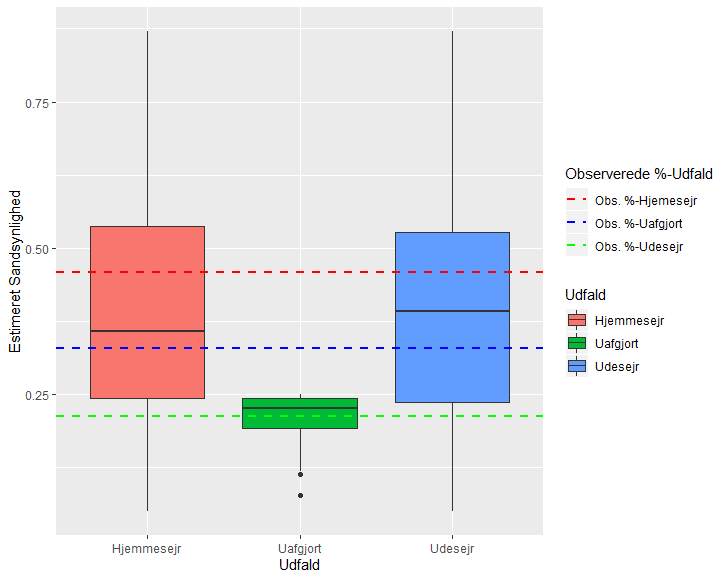
\includegraphics[width=\textwidth]{EstSSHStatisk.png}
    \caption{Boxplot af estimerede sandsynligheder mod udfald for den statiske model}
  \end{minipage}
  \\
  \begin{minipage}[b]{0.6\textwidth}
    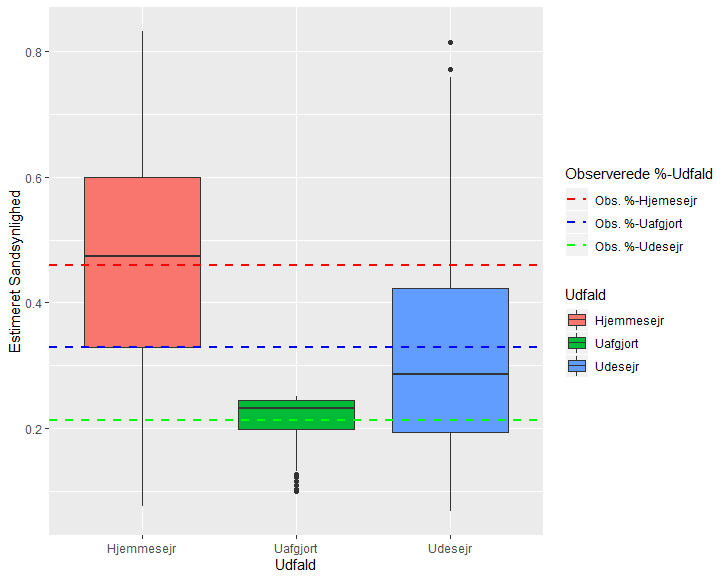
\includegraphics[width=\textwidth]{EstSSHDyn.png}
    \caption{Boxplot af estimerede sandsynligheder mod udfald for den dynamiske model}
  \end{minipage}
\end{figure}
 For at se nærmere på de estimerede sandsynligheder, kigger vi på deres respons-residualer mod de fittede værdier for de tre udfald; dette ses i Figure 3 og 4. Den sorte linje viser gennemsnittet af residualerne, og den røde linje er en kerneudglatning med båndbredden 0.06 for hjemme- og udesejr og 0.02 for uafgjort. \textcolor{blue}{Båndbredderne er valgt ved brug af \textit{R}-funktionen {\fontfamily{qcr}\selectfont dpill}, (som estimerer ud fra least squares, og udvælger bredden ud fra Mallows Cp)}. Det ses at middelværdierne for den dynamiske model er tættere på 0 end de er for den statiske. Den statiske model har en middelværdi over 0 for hjemmesejrs residualer og under 0 for udesejrs residualer. Dette er en forventelig følge, da den statiske model generelt vil overestimere sandsynligheden for udesejr og underestimere sandsynligheden for hjemmesejr. Der ser ikke ud til at danne sig noget klart mønster for de fittede værdier, dog er der noget støj ved halerne. Især ved de lave fittede værdier for hjemmesejr, ser det ud til at begge modeller har en tendens til at underestimere sandsynligheden, dette er dog meget vægtet af den ene observation i halen. Denne observation kommer fra en kamp mellem HOB og FCK i runde 30, hvor HOB vandt, på trods af, at styrken for FCK var markant større end styrken for HOB. Hvis denne observation blev fjernet, ville kerneudglatningen i den venstre hale være mere flad. Det samme er tilfældet for residualerne tilhørende udesejr for den statiske model, hvor der er en observation der stikker markant ud ved de høje fittede værdier. Det ser mere kritisk ud for residualerne til hjemmesejr for den dynamiske model, da vi får en stigning ved store fittede værdier. Dette er dog igen kun baseret på 3-4 observationer, og er derfor svært, at konkludere noget konkret ud fra. Residualerne tilhørende de uafgjorte kampe er meget ens for de to modeller, hvilket også måtte forventes, da $\theta$ er meget ens for dem. Der er dog en lidt større spredning \textcolor{blue}{for uafgjort} i de fittede værdier for den dynamiske model, hvilket skyldes \textcolor{blue}{forskellen i $\beta$'erne, og især implementeringen af hjemmebanefordelen}. Det er generelt svært at sige noget konkret om disse residualer, eftersom vi har så få observationer i hver kategori. Derfor vælger vi heller ikke at fjerne nogle af de outliers der er beskrevet.
\begin{figure}[ht]
  \centering
  \begin{minipage}[b]{0.5\textwidth}
    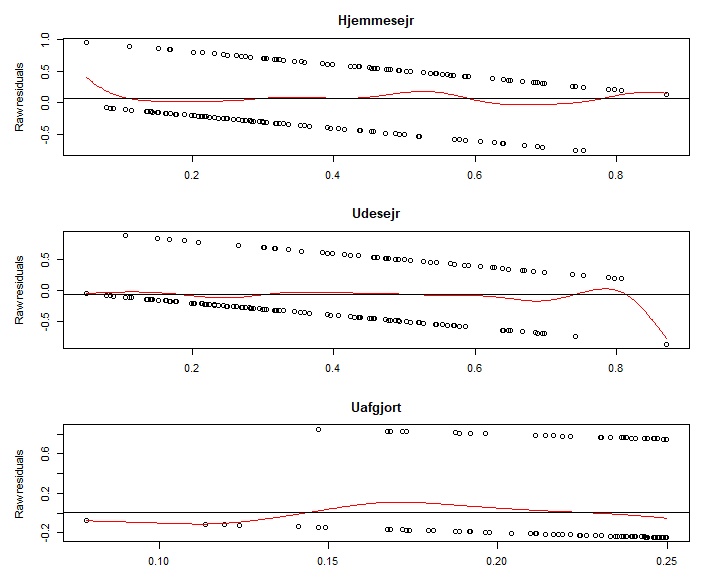
\includegraphics[width=\textwidth]{ResVsFitStat.png}
    \caption{Respons-residualer mod fittede værdier for den Statiske model}
  \end{minipage}
  \begin{minipage}[b]{0.5\textwidth}
    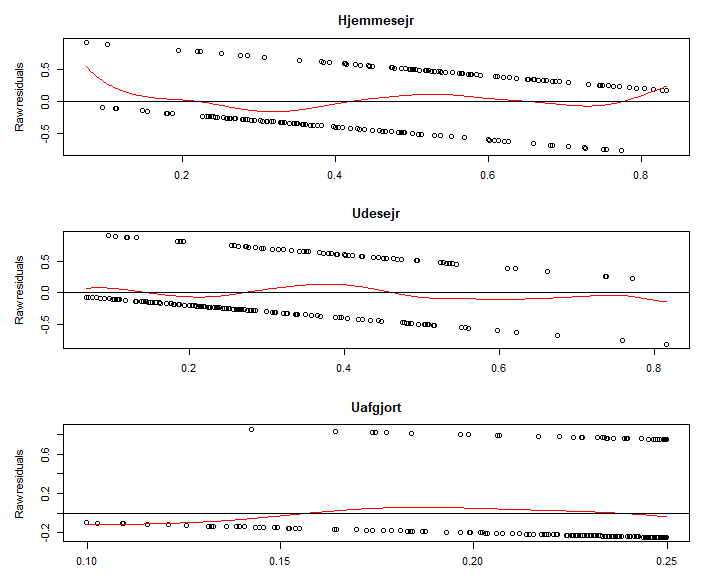
\includegraphics[width=\textwidth]{ResVsFitDyn.png}
    \caption{Respons-residualer mod fittede værdier for den dynamiske model}
  \end{minipage}
\end{figure}
\clearpage
\section{Shrinkage metoder}
\textcolor{blue}{Fortæl hvad idéen med implementering af lasso er. Fortæl at vi kun vil tage udgangspunkt i den dynamiske}
\textit{Shrinkage} metoders formål er i simpleste forstand, er at forbedre vores model ved at mindske modellens prædiktionsfejl. Det prædiktive element kommer af, at modellens parametre bliver estimeret ud fra et træningsdatasæt, for derefter at blive testet på et andet testdatasæt. Givet et datasæt med observationerne for $N=(n+q)$ spillerunder, kalder vi træningsdatasættet for $n$ og testdatasættet for $q$. En måde, at måle modellens prædiktionsfejl på er \textit{mean squarred prediction error} (MSPE): I MSPE udregnes den kvadrede prædiktionsfejl for hver af sandsynlighederne ($p_{i\cdot ij}, p_{j\cdot ij}, p_{0\cdot ij}$) individuelt, og MSPE for kampene mellem hold $i$ og hold $j$ for en given testperiode bliver så summen af prædiktionsfejlene for hver af de tre estimerede sandsynligheder. MSPE for at hold $i$ vinder over hold $j$ bliver:
\sout{Hvis vi har et givet datasæt med observationer for $N=(1,...,n,...,n+q)$ spillerunder, hvor modellens parametre bliver estimeret på et træningsdataset ($t=1,...,n)$, hvorefter prædiktionsfejlene bliver estimeret på et testdatasæt ($t=n+1,...,n+q$), hvor $q$ er antal tidspunkter (spillerunder) vi tester modellen på. Vi ønsker at teste vores model i forhold til to forskellige tabsfunktioner: \textit{mean squared prediction error} (MSPE) og en mere anvendt indenfor klassificeringsproblemer \textit{logistic loss} (log loss) også kendt som \textit{cross entropy loss}. }
\begin{align*}
\text{MSPE}\big{(}\hat{p}_{i\cdot ij}\big{)}=&E\Big{[}\big{(}y_{i\cdot ij}-\hat{p}_{i\cdot ij}\big{)}^2\Big{]}\\
=&E\Big{[}\big{(}\hat{p}_{i\cdot ij}-E\big{[}\hat{p}_{i\cdot ij}\big{]}+E\big{[}\hat{p}_{i\cdot ij}\big{]}-y_{i\cdot ij}\big{)}^2\Big{]}\\
=&E\Big{[}\big{(}\hat{p}_{i\cdot ij}-E\big{[}\hat{p}_{i\cdot ij}\big{]}\big{)}^2+2\big{(}\hat{p}_{i\cdot ij}-E\big{[}\hat{p}_{i\cdot ij}\big{]}\big{)}\big{(}E\big{[}\hat{p}_{i\cdot ij}\big{]}-y_{i\cdot ij}\big{)}\\
&+\big{(} E\big{[}\hat{p}_{i\cdot ij}\big{]}-y_{i\cdot ij}\big{)}^2\Big{]}\\
=&E\Big{[}\big{(}\hat{p}_{i\cdot ij}-E\big{[}\hat{p}_{i\cdot ij}\big{]}\big{)}^2\Big{]}
+2\underbrace{\big{(}E\big{[}\hat{p}_{i\cdot ij}\big{]}-E\big{[}\hat{p}_{i\cdot ij}\big{]}\big{)}}_{0}\big{(}E\big{[}\hat{p}_{i\cdot ij}\big{]}-y_{i\cdot ij}\big{)}\\
&+\big{(} E\big{[}\hat{p}_{i\cdot ij}\big{]}-y_{i\cdot ij}\big{)}^2\\
=&E\Big{[}\big{(}\hat{p}_{i\cdot ij}-E\big{[}\hat{p}_{i\cdot ij}\big{]}\big{)}^2\Big{]}+\Big{(} E\big{[}\hat{p}_{i\cdot ij}\big{]}-y_{i\cdot ij}\Big{)}^2\\
=&Var\Big{(}\hat{p}_{i\cdot ij}\Big{)}+\text{Bias}^2\Big{(}\hat{p}_{i\cdot ij}\Big{)},\\
\intertext{Vi ser altså, at prædiktionsfejlen er en funktion af den kvadrerede bias af vores estimator og variansen af vores estimator. \textcolor{blue}{For at minimalisere vores prædiktionsfejl ønsker vi dermed at minimalisere bias og varians.} MSPE for alle de estimerede udfald af kampene mellem hold $i$ og hold $j$ bliver:}
\text{MSPE}\big{(}\hat{p}_{ij}\big{)}&=\text{MSPE}\big{(}\hat{p}_{i\cdot ij}\big{)}+\text{MSPE}\big{(}\hat{p}_{j\cdot ij}\big{)}+\text{MSPE}\big{(}\hat{p}_{0\cdot ij}\big{)},\\
\intertext{og MSPE tabsfunktionen for hele modellen bliver:}
\mathcal{T}_{\text{MSPE}}\big{(}\hat{p}_{ij}\big{)}&=\frac{1}{h(h-1)/2}\sum_{i<j}\text{MSPE}\big{(}\hat{p}_{ij}\big{)},\\
\intertext{hvor $h(h-1)/2$ beskriver samtlige mulige opgør mellem to forskellige hold. Numerisk bliver MSPE tabsfunktionen for et givent træningsdatasæt $n$ og testdatsæt $q$:}
\mathcal{T}_{\text{MSPE}}\big{(}\hat{\beta}^{-q},\hat{\theta}^{-q}|x,y_{ij},n,q\big{)}&=\frac{1}{ak}\sum_{t\in q}\sum_{i<j}\big{(}y_{i\cdot ij}(t)-\hat{p}_{i\cdot ij}(t)\big{)}^2+\big{(}y_{j\cdot ij}(t)-\hat{p}_{j\cdot ij}(t)\big{)}^2+\big{(}y_{0\cdot ij}(t)-\hat{p}_{0\cdot ij}(t)\big{)}^2\Big{)},\\
\intertext{hvor $\hat{\beta}^{-q}, \hat{\theta}^{-q}$ viser at parametrene er estimeret uden observationerne fra testdatasættet $q$, og $ak$ betegner det totale antal kampe der ber bliver testet prædiktionsfejl for (antal kampe i q).}
\end{align*}
En anden mere hyppigt anvendt tabsfunktion i klassificeringsproblemer er \textit{logistic loss} (log loss) også kendt som \textit{cross entropy loss}. I log loss er den forventede størrelse for prædiktionsfejlen beregnet i forhold til hvor langt væk den estimerede sandsynlighed for det sande udfald er fra 1; log loss prædiktionsfejlen i en kamp mellem hold $i$ og hold $j$ i runde $t$ bliver:
\begin{align*}
    \mathcal{T}_{\text{MSPE}}\big{(}p_{ij}(t)\big{)}&=-\Big{(}y_{i\cdot ij}(t)\log\big{(}\hat{p}_{i\cdot ij}(t)\big{)}+y_{j\cdot ij}(t)\log\big{(}\hat{p}_{j\cdot ij}(t)\big{)}+y_{0\cdot ij}(t)\log\big{(}\hat{p}_{0\cdot ij}(t)\big{)}\Big{)},\\
\intertext{og log tabsfunktionen for hele testsættet bliver:}
\mathcal{T}_{\log}\big{(}\hat{\beta}^{-q},\hat{\theta}^{-q}|x,y_{ij},n,q\big{)}&=-\sum_{t\in q}\sum_{i<j}\Big{(}y_{i\cdot ij}(t)\log\big{(}\hat{p}_{i\cdot ij}(t)\big{)}+y_{j\cdot ij}(t)\log\big{(}\hat{p}_{j\cdot ij}(t)\big{)}+y_{0\cdot ij}(t)\log\big{(}\hat{p}_{0\cdot ij}(t)\big{)}\Big{)}.\\
\intertext{Ved at sammenligne med likelihood funktionen ser vi, at minimalisere log tabsfunktionen er ækvivalent med at minimalisere den negative log likelihood funktion over testsættet:}
-\ell\big{(}\hat{\beta},\hat{\theta}\big{)}&=-\log\prod_{t\in q}\prod_{i<j}\hat{p}_{i\cdot ij}(t)^{y_{i\cdot ij}(t)}\hat{p}_{j\cdot ij}(t)^{y_{j\cdot ij}(t)}\hat{p}_{0\cdot ij}(t)^{y_{0\cdot ij}(t)}\\
&=-\sum_{t\in q}\sum_{i<j}\Big{(}y_{i\cdot ij}(t)\log\big{(}\hat{p}_{i\cdot ij}(t)\big{)}+y_{j\cdot ij}(t)\log\big{(}\hat{p}_{j\cdot ij}(t)\big{)}+y_{0\cdot ij}(t)\log\big{(}\hat{p}_{0\cdot ij}(t)\big{)}\Big{)}.
\end{align*}

\subsection{Lasso}
\textit{"Sometimes, less is more." - William Shakespeare.}\\
Indtil videre har vi anvendt samtlige af de forklarende variable, til at beskrive de forskellige holds styrker. Der er altså en risiko for, at vi overfitter vores model med overflødige variable, som enten beskriver; den samme varians, beskriver den dårligt, eller slet ikke beskriver den. I dette afsnit vil vi tage udgangspunkt Shakespeare's citat, og forsøge at indskærpe modellen, så de "bedste" variable vægtes mest og de dårligere enten vægtes mindre eller fjernes helt. Robert Tibshirani (1996) foreslår en metode kaldet lasso \textit{(least absolute shrinkage and selection operator)} til at identificere, hvor godt de forskellige parametre beskriver udfaldene og justerer koefficienter derefter. Lasso-optimeringsproblemet tager som tidligere udgangspunkt i maksimere likelihooden eller ligeledes minimere den negative log-likelihood, under en bibetingelse:
\begin{align*}
&\min_{\beta,\,\theta} \Big{\{}-\ell(\beta,\theta)\Big{\}} \\
&\text{u.b.b. }\sum_{i=1}^k|\beta_i|\leq s,
\end{align*}
hvor bibetingelsen straffer optimeringsproblemet i forhold til $\beta$-koefficienterne, og $s$, som beskriver den størst mulige sum af $\beta$-koefficienterne, er en brugervalgt strafparameter. 
Vi opskriver lasso-problemet på \textit{Lagrange-form}, da vi senere hen benytter dets praktiske anvendelighed:
\begin{align*}
\min_{\beta,\,\theta} \Big{\{}-\ell(\beta,\theta)+\lambda\sum_{i=1}^k|\beta_i|\Big{\}},
\end{align*}
hvor $\lambda\geq0$ er en strafparameter tilsvarende $s$, og beskriver størrelsen på denne straf. $\lambda$ og $s$ har et inverst forhold, så når $\lambda$ er høj, er $s$ lav.\textcolor{red}{SE OM VI KAN FINDE SAMMENHÆNG} Hvis $s\geq\sum_i^k\|\beta_i|\iff \lambda=0$ vil lasso løsningen være lig maksimum likelihood løsningen, men hvis $s=\frac{1}{\delta}\sum_i^k\|\beta_i|$ vil koefficienterne gennemsnitligt mindskes til $\frac{1}{\delta}$ af hvad de var før.
\subsubsection{Estimation af lasso-parametre}
\textcolor{blue}{For at forklare effekten af lasso på parametrene, vil vi tage udgangspunkt i en lineær model med ortogonal designmatrice, fordi vi så kan skrive resultatet af lasso ned eksplicit. Når X er ortogonal er $X^T=X^{-1}$, så mindste kvadraters løsningen bliver:}
\begin{align*}
\hat{\beta}=\big{(}X^TX\big{)}^{-1}X^Ty=X^Ty.
\end{align*}
Lasso-problemet for en lineær model bliver:
\begin{align*}
&\min_\beta \Big{\{}\big{(}y-X\beta\big{)}^T\big{(}y-X\beta\big{)}+\lambda\sum_{i=1}^k|\beta_i|\Big{\}}=\min_\beta \Big{\{}y^Ty+X^TX\beta^T\beta-2y^TX\beta+\lambda\sum_{i=1}^k|\beta_i|\Big{\}},\\
\intertext{thi $y^Ty$ er uafhængig af $\beta$, $X^TX=1$ og $\hat{\beta}=X^Ty$ kan vi omskrive problemet til:}
&\min_\beta \Big{\{}2\beta^2-\hat{\beta}\beta+\lambda\sum_{i=1}^k|\beta_i|\Big{\}}=\min_\beta \Big{\{}\sum_{i=1}^k\Big{(}2\beta_i^2-\hat{\beta_i}\beta_i+\lambda |\beta_i|\Big{)}\Big{\}}.\\
\intertext{Objektfunktion er nu en sum af k identiske problemer, som kan løses hver for sig. Vi tager udgangspunkt i det i'te problem, og får objektfunktionen:}
&f(\beta_i)=-2\hat{\beta}_i\beta_i+\beta_i^2+\lambda|\beta|.\\
\intertext{Thi vi ønsker at minimere objektfunktionen må det gælde, at $\hat{\beta}_i>0\rightarrow\beta_i\geq0$, for ellers ville objektfunktionen kunne mindskes ved at skifte fortegnet for $\beta_i$, og ligeledes må det gælde, at $\hat{\beta}_i<0\rightarrow\beta_i\leq0$ Ved at differentier og sætte lig 0 fås den afledte:}
&f'(\beta_i)=-2\text{Fortegn}\big{(}\hat{\beta_i}\big{)}\hat{\beta_i}+2\beta_i+\lambda. \\
\intertext{Ved at isolere $\beta_i$ og gange begge sider med fortegnet for $\beta_i$ (fortegnet for $\hat{\beta_i}$), for at sikre positivt fortegn på venstre siden, fås:}
&\beta_i=\text{Fortegn}\big{(}\hat{\beta_i}\big{)}\Big{(}\text{Fortegn}\big{(}\hat{\beta_i}\big{)}\hat{\beta_i}-\frac{1}{2}\lambda\Big{)}=\text{Fortegn}\big{(}\hat{\beta_i}\big{)}\big{(}|\hat{\beta_i}|-\frac{1}{2}\lambda\big{)},\\
\intertext{hvis $\hat{\beta}_i<0$ kræves, at $\text{Fortegn}\big{(}\hat{\beta_i}\big{)}\big{(}|\hat{\beta_i}|-\frac{1}{2}\lambda\big{)}\leq0$ og ligeledes kræver $\hat{\beta}_i>0$, at $\text{Fortegn}\big{(}\hat{\beta_i}\big{)}\big{(}|\hat{\beta_i}|-\frac{1}{2}\lambda\big{)}\geq0$, hvilket løses ved at sætte $\big{(}|\hat{\beta_i}|-\frac{1}{2}\lambda\big{)}$ lig nul, hvis ledet er negativt:}
&\hat{\beta}_i^{\text{lasso}}=\text{Fortegn}\big{(}\hat{\beta_i}\big{)}\big{(}|\hat{\beta_i}|-\frac{1}{2}\lambda\big{)}^{+}
\end{align*}
Vi ser tydeligt, at når $\lambda$ stiger, går $\hat{\beta}_i^{\text{lasso}}$ mod 0, samt at $\lambda\geq2|\hat{\beta}_i|\rightarrow \hat{\beta}_i^{\text{lasso}}=0$. Det vil sige, at i forbindelse med at $\lambda$ stiger vil lasso-estimaterne gå mod 0, samt at når $\lambda$ bliver tilpas stor vil en eller flere koefficienter sættes lig 0, hvilket betyder at lasso løbende træffer et valg af underum. Idéen er nu, at når $|\beta|$-koefficienterne mindskes, mindskes variansen af de estimerede sandsynligheder, hvilket medfører at modellens prædiktionsfejl mindskes. Dette sker dog på bekostning af, at når $|\beta|$-koefficienterne mindskes, medfører det også at den kvadrerede bias stiger, hvilket øger modellens forventede fejl. Variansen falder, da sandsynlighederne bliver mindre påvirket af deres kovariater. Den kvadrerede bias stiger, da lasso trækker estimaterne mod 0 og væk fra de centrale løsninger. Ved justering af $\lambda$ bliver modellens forventede prædiktionsfejl altså trukket i hver sin retning på grund af ændringer i bias og varians. Dette forhold mellem bias og varians kaldes \textit{The Bias-Variance Decomposition} (ref. ESL). Humlen er så, at finde det $\lambda$ der minimerer den forventede prædiktionsfejlene i modellen.
\sout{
Det ses tydeligt, at når $\lambda$ stiger, falder $\hat{\beta}^{\text{lasso}}$, samt at $\lambda=2X^Ty\rightarrow \hat{\beta}^{\text{lasso}}=0$. Det vil sige, at i forbindelse med at $\lambda$ stiger vil $\beta$-koefficienterne mindskes, samt at når $\lambda$ bliver tilpas stor vil en eller flere koefficienter sættes lig 0, hvilket betyder at lasso løbende træffer et valg af underum. Idéen er nu, at når $\beta$-koefficienterne mindskes, mindskes variansen af de estimerede sandsynligheder, hvilket medfører at modellens forventede fejl i forudsigelserne mindskes. Dette sker dog på bekostning af, at når $\beta$-koefficienterne mindskes, medfører det også at den kvadrerede bias stiger, hvilket øger modellens forventede fejl. Variansen falder, da sandsynlighederne bliver mindre påvirket af deres kovariater. Den kvadrerede bias stiger, da lasso trækker estimaterne mod 0 og væk fra de centrale løsninger. Ved justering af $\lambda$ bliver modellens forventede prædiktionsfejl altså trukket i hver sin retning på grund af ændringer i bias og varians. Dette forhold mellem bias og varians kaldes \textit{The Bias-Variance Decomposition} (ref. ESL). Humlen er så, at finde det $\lambda$ der minimerer de forventede fejl i modellen.}\\ 
I den dynamiske model med lasso-straf, bliver sandsynligheden for, at hold $i$ vinder over hold $j$ til tidspunkt $t$:\\
\begin{align}
    p_{i\cdot ij}(t)=P\big{\{}Y_{i}(t)>Y_{j}(t)\big{\}}=\frac{1}{1+e^{-\big{(}x_i^T(t,\alpha)\beta(\lambda)-x_j^T(t,\alpha)\beta(\lambda)-\eta\big{)}}},
\end{align}
\subsection{Karush-Kuhn-Tucker}
Lasso og ridge problemerne, er ikke-lineære problemer og løses ved hjælp Karush-Kuhn-Tucker betingelserne; eksempel med lasso, hvor $g(\beta)=\Big{(}\sum_i^k\|\beta_i\| \Big{)}$ er KKT betingelserne i optimum for minimeringsproblemet:
\begin{align}
    -\frac{\partial\ell(\beta,\theta)}{\partial\beta}+\lambda\frac{\partial g(\beta)}{\partial \beta}&=0\\
    -\frac{\partial\ell(\beta,\theta)}{\partial\theta}&=0\\
    \lambda&\geq 0 \;\;(\lambda=0\text{ hvis }s\geq\sum_i^k\|\beta_i\|)
\end{align}\\
Løsningen til KKT problemerne bliver illustreret fremragende af i Figure 1: \\
\begin{center}
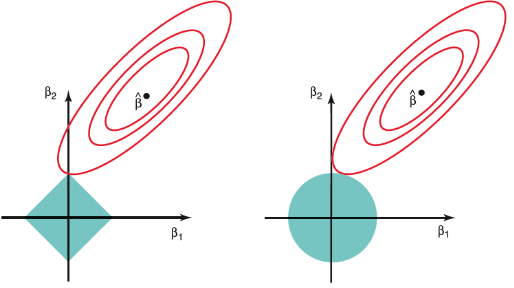
\includegraphics[scale=0.8]{GLR.PNG}   
\end{center}
\textit{\#Plagiat? Illustrationen til venstre er lasso, og illustrationen til højre er ridge. Problemerne er illustreret med 2 beskrivende variable, hvor $\hat{\beta}$ er maksimum likelihood estimaterne, hvis der ikke bliver straffet. De grønne arealer illustrere bibetingelserne; de mængder som løsningen befinder sig i, efter at der er tilføjet et strafled. De røde cirkler illustrere forskellige likelihood værdier, og mindskes jo længere væk fra centrum punktet befinder sig.løsningerne på problemerne at at vælge det punkt i de grønne mængderne der kommer tættest på ML løsningen. Lasso problemet har hjørner, og hvis løsningen er på et hjørne, som på figuren, er der kun et aktivt parameter.}
\subsection{Implementering af lasso}
Til at implementere lasso-straffen, approksimerer vi strafledet med en glat udgave, \textcolor{blue}{hvorved vi sørger for at den er differentiabel}, $\lambda |\beta| = \lambda(\sqrt{\beta^2+c^2})$ hvor vi lader $c\rightarrow 0$. Vi kan dermed ikke antage at vores estimerede \textcolor{blue}{parameterkoefficienter} bliver lig 0, og derfor sætter vi en grænse for hvor tæt de må være på 0, før vi fjerner dem. Denne grænse skal selvfølgelig være så lav at det giver mening at fjerne dem, hvorfor vi vælger at sætte $\beta_k$ lig 0 og dermed fjerne den når $\beta_k<10^{-6}$. Efter vi har fjernet en parameter, skal likelihooden med lasso-straffen selvfølgelig i løbet af de følgende iterationer blive større, end før vi fjernede parametren. For at kunne sammenligne kovariaternes størrelser på tværs af hinanden, standardiserer vi designmatricen. Dette gøres ved at skalere hver række, så middelværdien er lig 0 og variansen er lig 1, dermed bliver det $i$'te element i den $j$'te række i designmatricen opskrevet ved 
\begin{align*}
    Standard(x_{ji}) &= \frac{x_{ji}-\frac{1}{h}\sum_{i=1}^h{x_{ji}}}{\sqrt{\frac{1}{h}\sum_{i=1}^h(x_{ji}-\Bar{x}_j)^2}}=\frac{x_{ji}-\Bar{x}_j}{\sigma_j}
\end{align*}
For at sikre at likelihooden konvergerer (når den er i mængden der opfylder \textbf{Theorem 9.1.6}) \textcolor{blue}{(s. 249 K.P.M (2012))}, skal vi for hvert skridt i Newton-Raphson finde en skridtlængde, $\omega$, der opfylder:\\
\begin{align*}
    v_{k+1} &= v_{k} -  i(\beta_k,\theta_k)^{-1}g(\beta_k,\theta_k)\omega,\\
    \ell(v_{k}) &< \ell(v_{k+1}).
\end{align*}
Dette gør vi ved brug af \textit{line search}, som foreslået af Kevin P. Murphy (2012). Her kan problemet opskrives som 
$\max_{\omega \in \mathcal{N}} \ell(v_{k+1})$, hvor vi i vores tilfælde vælger 
$\mathcal{N} = \{1,\frac{1}{2},...,\frac{1}{100}\}$. Vi tester dermed skridtlængderne i faldende orden, hvor $\omega$ vælges for det første tilfælde der opfylder betingelsen $\ell(v_k)<\ell(v_{k+1})$. Algoritmen til at estimere parametrene med lasso-straf, kan læses som pseudokode i \textit{Algorithm 3}\\
\begin{algorithm}[H]
\SetAlgoLined
\KwResult{$\min_{\beta,\,\theta} \Big{\{}-\ell\Big{(}\beta,\theta|x,y_{ij}(t),r_{ij}(t)\Big{)}\Big{\}}$}
 Initialisér $v_0 = \begin{bmatrix}
           \beta \\
           \theta
         \end{bmatrix} =\begin{bmatrix}
           \beta_0 \\
           \theta_0
         \end{bmatrix}\;$\\
 \For{($k = 1,2,... $ indtil konvergens)}{
  \For{$(t = 3,t\leq SlutRunde,t++)$}{
        \eIf{($\alpha\geq t$)}{$\alpha_1 = t-1\;$}{$\alpha_1 = \alpha\;$}
        $L(\beta_k,\theta_k) = \sum_{c = t-\alpha_1}^{t-1}\sum_{i<j}\ell\Big{(}\beta,\theta\Big{|}x(t,\alpha),Y_{ij}(t),R_{ij}(t)\Big{)}$\;
        $g_k = g_k + \nabla \L\Big{(}\beta_k,\theta_k\Big{)}$\;
        $j_k = j_k + (-\nabla^2 L\Big{(}\beta_k,\theta_k\Big{)})$\;
    }
\For{(\mathcal{N} = 1:100)}{
   $\omega = \frac{1}{\text{\mathcal{N}}}$\;
   $v_{k+1} = v_k - j_k^{-1}g_k\omega$\;
   $\begin{bmatrix}
       \beta_{k+1} \\
       \theta_{k+1}
    \end{bmatrix} = v_{k+1}$\;
        \If{$L(\beta_{k+1},\theta_{k+1})>L(\beta_k,\theta_k)$}
        {\textbf{break}\;}
        
    }
 }
\caption{Newton-Raphson for Dynamisk Model med lasso-straf}
\end{algorithm}
\subsection{Lasso-Algoritmer}
\section{Modelovervejelser og udvælgelse}
\subsection{Krydsvalidering}
For at udvælge størrelsen af vores strafparameter $\lambda$ vil vi benytte os af krydsvalidering, som bruges til sammenligne prædiktionsfejlene for modellen for forskellige $\lambda$ værdier. Krydsvalidering fungerer ved at benytte dele af den givne datamængde til at konstruere modellen, og andre dele til teste modellen: Vi deler datamængden op i $Q$ lige store dele, hvor vi lader $q\in \{1,...,Q\}$ betegne de forskellige delmægnder; Dermed kan vi nu skrive det fulde datasæt som: $N=(1,..,Q)$. Vi fitter nu vores model til det fulde datasæt minus den $q$'te delmængde, så dataen vi fitter vores model udfra, bliver: $n_{-q}=N-q$, hvorefter vi tester prædiktionsfejlene for den $q$'te udeladte testmængde. Denne test bliver så gentaget $Q$ gange, hvor hver af delmængderne bliver anvendt som testmængde én gang. Krydsvaliderings prædiktionsfejlen bliver så et gennesnit af alle prædiktionsfejlene for hver af de $N$ spillerunder:
\begin{align*}
KV\big{(}\ell(\hat{\beta},\hat{\theta})\big{)}&=\frac{1}{N}\sum_{q=1}^Q\mathcal{T}\big{(}\hat{\beta}^{-q},\hat{\theta}^{-q}\big{)}\\
\end{align*}
\textcolor{blue}{Den grafiske fremstilling af ridge (Side 65 i ESL) skal vi lave for de modeller vi vælger at lave... den er lækker}
\clearpage
\section{Appendix}
\subsection{Appendix A - Tabeller uden afrunding}
\begin{table}[ht]
\centering
\begin{adjustbox}{max width=\textwidth}
\begin{tabular}{|l|rr|rr|}
\hline
\multicolumn{1}{|l|}{} & \multicolumn{2}{l|}{Statisk Model} & \multicolumn{2}{l|}{Dynamisk Model} \\
\hline
Parameter & Estimat & SE & Estimat & SE \\
  \hline
    $\hat{\beta}_1$ & - & - & 0.317114 & 0.144718\\
    $\hat{\beta}_2$ & - & - & -0.175658 & 0.111606\\
    $\hat{\beta}_3$ & 0.147326 & 0.393619 & 0.086457 & 0.086439\\
    $\hat{\beta}_4$ & 0.227893 & 1.010051 & 0.108508 & 0.215125\\
    $\hat{\beta}_5$ & -0.237965 & 0.809342 & -0.143969 & 0.225400\\
    $\hat{\beta}_6$ & -0.007531 & 0.076213 & 0.048565 & 0.032032\\
    $\hat{\beta}_7$ & -0.029734 & 0.041813 & -0.016217 & 0.020832\\
    $\hat{\beta}_8$ & -0.012030 & 0.140722 & 0.000034 & 0.000100\\
    $\hat{\beta}_9$ & -0.020433 & 0.069996 & -0.019022 & 0.037623\\
    $\hat{\beta}_{10}$ & -0.169596 & 0.441762 & 0.027197 & 0.137985\\
    $\hat{\beta}_{11}$ & 0.437399 & 1.870163 & -0.363863 & 0.241769\\
    $\hat{\beta}_{12}$ & -0.025784 & 0.256451 & -0.053460 & 0.102694\\
    $\hat{\theta}$ & 1.666758 & 0.121130 & 1.666445 & 0.123939\\
   \hline
\end{tabular}
\end{adjustbox}
\end{table}
\printbibliography %Printer referencer

\end{document}